\documentclass[12pt,letterpaper]{article}
\usepackage[body={18cm, 25cm}]{geometry}
\usepackage[utf8]{inputenc}
\usepackage{paralist}
\usepackage[english]{babel}
\usepackage{multicol}
\usepackage{multirow}
\usepackage{float}
\usepackage{amsmath}
\usepackage{mathtools}
\usepackage{amsfonts}
%\usepackage{amssymb}
\usepackage{graphicx}
\usepackage{geometry}
\usepackage{natbib}
\usepackage{subfig}%%Para incluir subgraficos
\geometry{verbose,letterpaper,tmargin=3cm,bmargin=2cm,lmargin=2cm,rmargin=2cm}
\usepackage{tabularx}
\usepackage{tabulary}
\usepackage[table]{xcolor}
\usepackage{authblk}
\usepackage{physics} % Extra operators and cool stuff
\usepackage[pdftex, pdftitle={Manual DAMIAN_par}, pdfauthor={Juan Gomez}, pdfsubject={Elastodynamics}, pdfkeywords={ wave propagation, computational mechanics, finite element analysis}, pdfpagemode=UseOutlines,bookmarks,bookmarksopen,pdfstartview=FitH,colorlinks,linkcolor=blue, urlcolor=black, citecolor=blue]{hyperref} %%Para incluir detalles cucas del pdf
\usepackage[ruled]{algorithm2e} % Include algorithms



\title{\textbf{WAVES: Explicit Parallelized Finite Element Solver for Wave Propagation Analysis}}


\author{Juan Gomez and Juan Carlos Vergara}
\usepackage{cleveref}
\begin{document}
\maketitle
\section{Introduction}
Topographic effects have been shown to play a major role in the determination of the seismic ground motions at a site. In the idealized case of homogeneous media submitted to horizontally polarized shear waves there is a relatively large family of analytic or semi-analytic frequency domain solutions. However in the more general case of in-plane waves or in actual three-dimensional topographies the problem needs to be solved numerically. In particular, algorithms based upon the finite element method (FEM) have the advantage of allowing the incorporation of arbitrary boundary conditions and material models. This article describes the explicit finite element code {\bf WAVES} which  has been created as part of the research program on topographic effects conducted at the research lab Grupo de Mecanica Aplicada at Universidad EAFIT. Although the code has been originally implemented for the solution of plane wave scattering problems in the time domain, it is also possible to conduct analysis of generalized dynamic problems in 2D and 3D domains. 

In simple terms the computer program finds the displacement time history for arbitrary two-dimensional and three-dimensional domains discretized into finite elements.  As its main features the code allows to conduct plane wave analysis using as input excitation the domain reduction (DRM) technique formulated by \cite{bielak2003}, while the time discretization corresponds to a central difference scheme (having diagonal mass matrices) with uncoupled equations for each degree of freedom. 

In the first part of the report we focus on the theoretical aspects of the DRM approach, including the formulation of the elastodynamics scattering problem. This theoretical discussion is presented directly in matrix form assuming that the reader is experienced with finite element algorithms. Following the discussion of the DRM method we present the time-domain discretization resulting in an explicit solution scheme. In part 4 of the report we describe the most relevant structural aspects of the program with particular emphasis on the addition of user defined finite elements and material models. In the final part of the report we show the model creation process using as study problem the case of a rectangular-shaped canyon embedded in an elastic half-space. Since the model involves a large number of elements the required input files are created with the aid of third party software.


\section{Formulation of the plane wave scattering problem}
\subsection*{Classical formulation of the scattering problem}

In order to have a general context of the physical basis of the DRM technique formulated by \cite{bielak2003} it is convenient to describe the so-called scattering problem in elastodynamics. We will use an integral equation approach based on the elastodynamics representation theorem \citep{vara1976}. The physical problem is schematized by the top part of \cref{fig:class part} which depicts a generalized half-space with domain $\Omega^+$ supporting a scatterer with domain $\Omega$. Both domains are bounded through the perfectly coupled surface $\Gamma$ and the remote boundary of the half-space $\Gamma^+$. Notice that the scatterer also comprises a localized, small-scale topographic feature (e.g., a microzone) embedded into a large topographic irregularity. The scattering problem consists in determining the response of the system when it is submitted to the action of an incident wave.

The domain reduction method, originally formulated by \cite{bielak2003} and verified in \cite{yoshimura2003domain} is a two-step algorithm developed for the simulation of earthquake ground motions in seismic scenarios containing strong variations in wavelength. The fundamental principle underlying the method is the classical partition of the field used in the formulation of scattering problems \citep{vara1976, courant2008methods, Bielak1984} written like ;

\begin{equation}
\label{free field}
{u}={u^0}+{w}
\end{equation}

\begin{figure}[H]
\centering
\subfloat{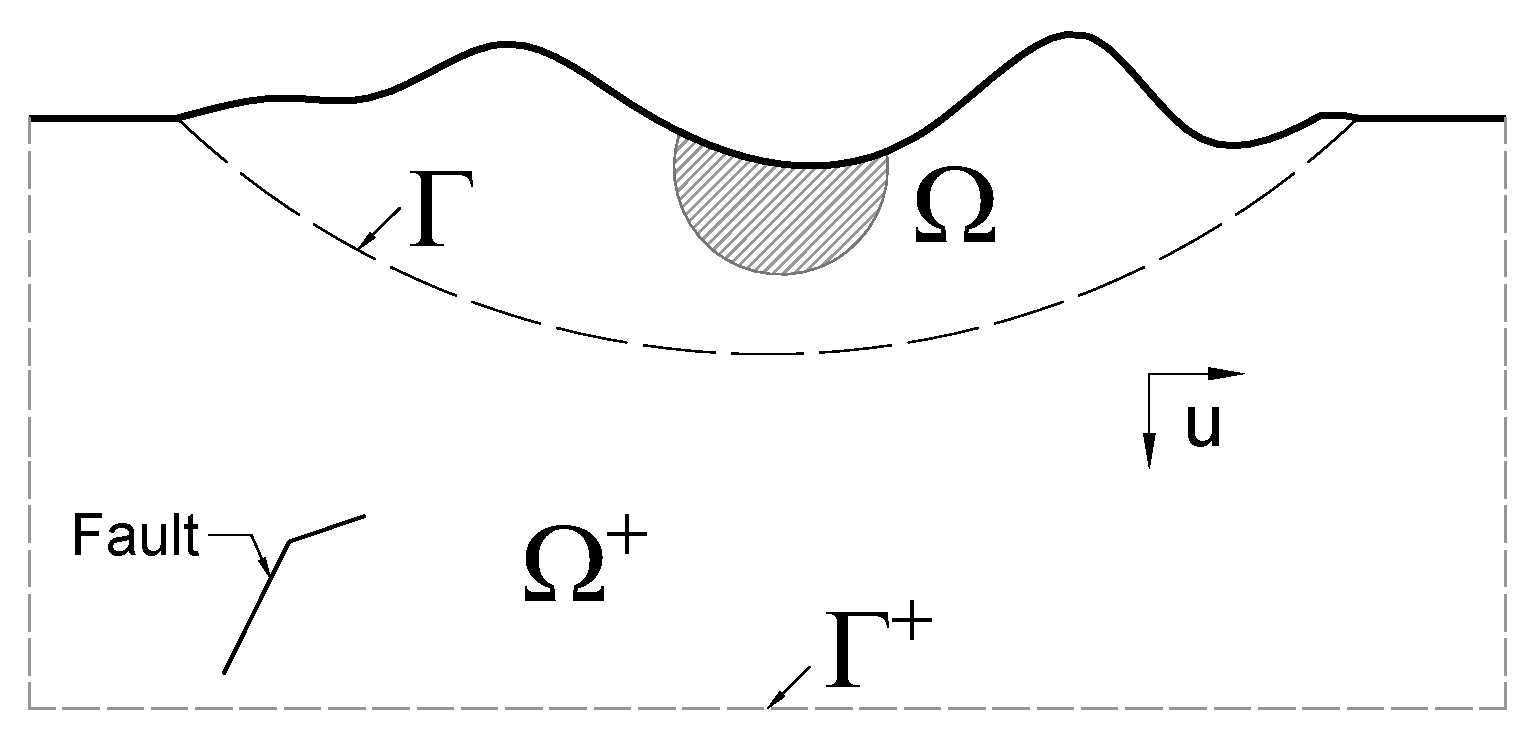
\includegraphics[width=3 in]{images/CLASSIC0.pdf}}
\subfloat{
\includegraphics[width=0.25 in]{images/equal.pdf}}\\
\subfloat{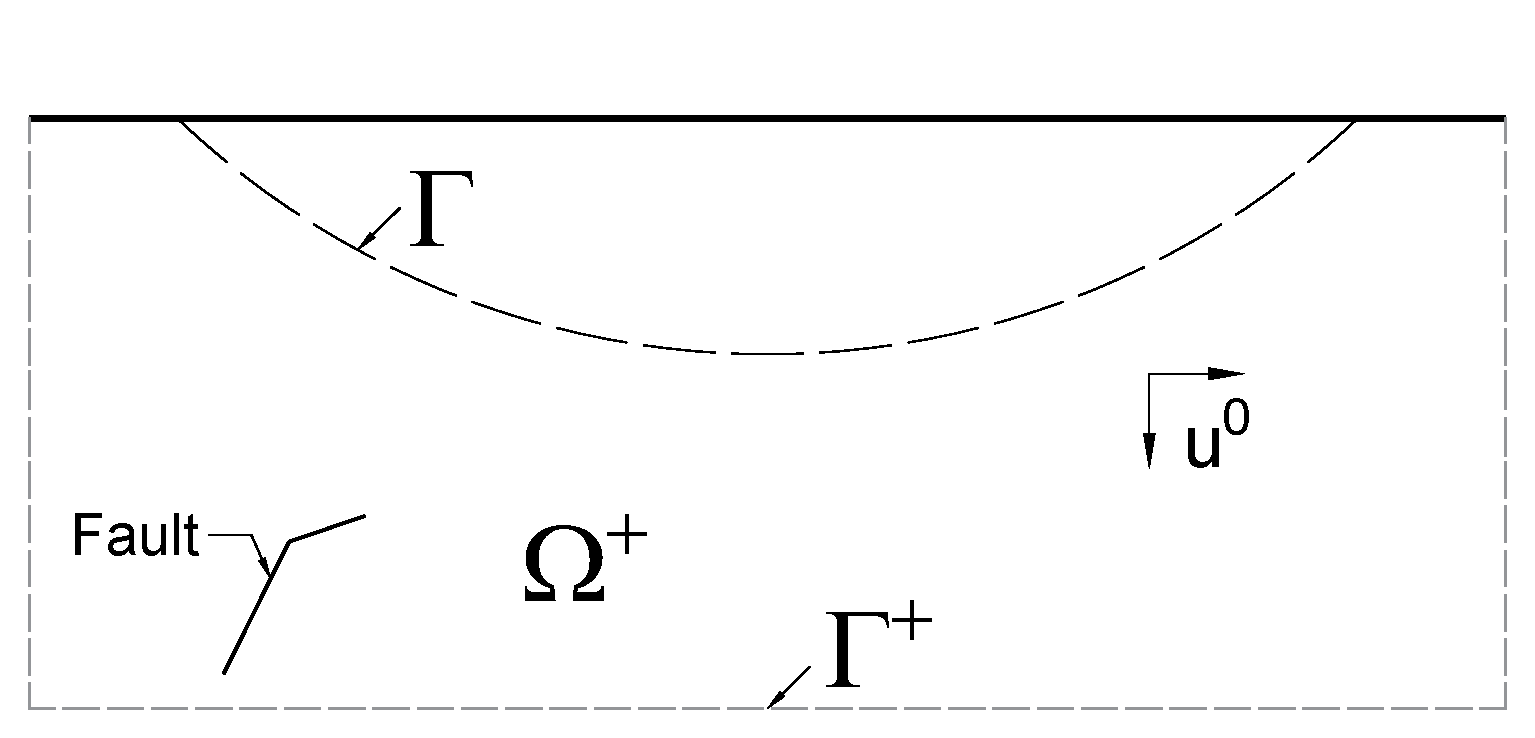
\includegraphics[width=3 in]{images/CLASSIC1.pdf}}
\subfloat{
\includegraphics[width=0.25 in]{images/plus.pdf}}
\subfloat{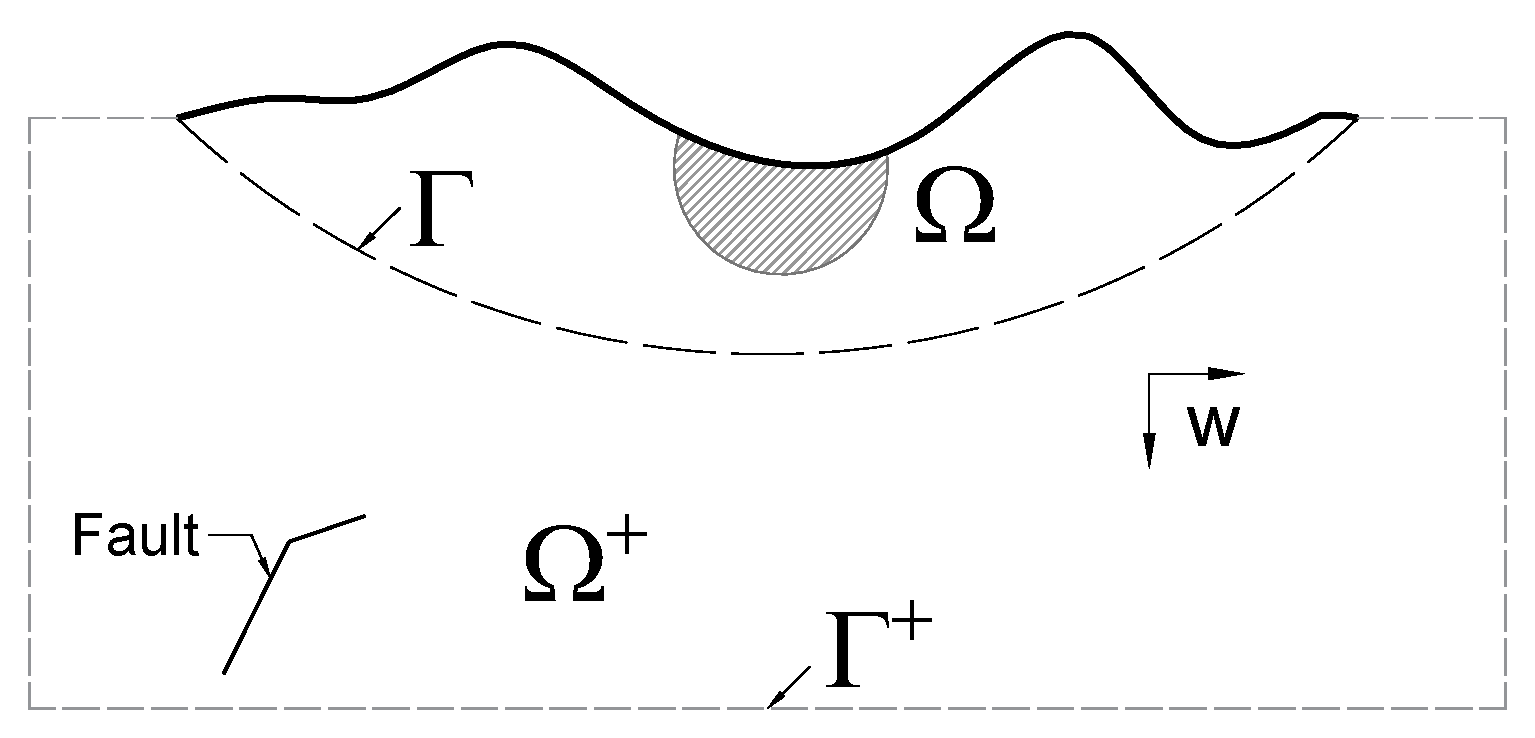
\includegraphics[width=3 in]{images/CLASSIC2.pdf}}
\caption{Partition of the field in the classical definition of the scattering problem. The free-field $u^0$ corresponds to the response of the half-space with the scatterer being removed (bottom left), while the scattered field $w$ would be the additional displacement introduced in the half-space once the scatterer $\Omega$ is considered (bottom right).}
\label{fig:class part}
\end{figure}

where ${u^0}$ is the free field motion or response of the half-space in the absence of the scatterer and ${w}$ is a scattered field or relative displacement motion between the total and free-field motion. This free field motion can be obtained in closed-form depending on the nature of the half-space and of the seismic excitation. In the more general case it is also found numerically from the solution of the simpler problem described in the bottom left of \cref{fig:class part}.

Following the elastodynamics representation theorem the boundary value problem for the total field inside the scatterer is governed by the integral equations;

\begin{equation}
{C_{ij}}(\vec \xi ){u_j}(\vec \xi ) = \int\limits_\Gamma  {G_{ij}^{FS}(\vec x;\vec \xi )} {t_j}(\vec x)dS(\vec x) - \int\limits_{\Gamma^+ + \Gamma } {H_{ij}^{FS}(\vec x;\vec \xi )} {u_j}(\vec x)dS(\vec x) \quad \text{for $\vec{\xi}$ inside $\Gamma^+ \cup \Gamma$}
\label{Vara 1}
\end{equation}

and where $G_{ij}^{FS}$ and $H_{ij}^{FS}$ are the full-space displacements and tractions Green's tensors respectively while $C_{ij}$ is a tensor which depends on the smoothness of the boundary and $u_i$ and $t_i$ are the total displacements and tractions vectors. Similarly, the relative motion in the half-space $w_i$ is governed by;

\begin{equation}
{C_{ij}}(\vec \xi ){w_j}(\vec \xi ) = \int\limits_\Gamma  {G_{ij}^{HS}(\vec x;\vec \xi )} t_j^w(\vec x)dS(\vec x) - \int\limits_\Gamma  {H_{ij}^{HS}(\vec x;\vec \xi )} {w_j}(\vec x)dS(\vec x) \quad \text{for $\vec{\xi}$ inside $S_F \cup \Gamma^+ \cup \Gamma$}
\label{Vara 2}
\end{equation}

where now $G_{ij}^{HS}$ and $H_{ij}^{HS}$ are the corresponding Green's tensors for the half-space. Notice that the excitation enters into the problem once the surface compatibility conditions;

\begin{equation} \label{comp}
\begin{split}
{u}& ={u^0}+{w}\\
{t}&+{t^0}+{t_w}=0
\end{split}
\end{equation}

are imposed along $\Gamma$.

\subsection*{Bielak et al(2003) DRM algorithm}
\addcontentsline{toc}{subsection}{Bielak et al(2003) DRM algorithm}
The problem is schematized by the top part of \cref{fig:bielak} which depicts a generalized half-space with domain $\Omega^+$ supporting a scatterer $\Omega$. Both domains are bounded through the perfectly coupled surface $\Gamma$. Notice that the scatterer comprises also a localized, small-scale topographic feature (e.g., a microzone) embedded into a large topographic irregularity. The relevant degrees of freedom have been labeled after \cite{bielak2003}. In this work we are interested in conducting SRA at the microzone.


The partitioned equations of motion for the half-space and scatterer (i.e., $\Omega$) read;


\begin{equation}
\left[ {\begin{array}{*{20}{c}}
{M_{ii}^\Omega }&{M_{ib}^\Omega }\\
{M_{bi}^\Omega }&{M_{bb}^\Omega }
\end{array}} \right]\left\{ {\begin{array}{*{20}{c}}
{{{\ddot u}_i}}\\
{{{\ddot u}_b}}
\end{array}} \right\} + \left[ {\begin{array}{*{20}{c}}
{K_{ii}^\Omega }&{K_{ib}^\Omega }\\
{K_{bi}^\Omega }&{K_{bb}^\Omega }
\end{array}} \right]\left\{ {\begin{array}{*{20}{c}}
{{u_i}}\\
{{u_b}}
\end{array}} \right\} = \left\{ {\begin{array}{*{20}{c}}
0\\
{{P_b}}
\end{array}} \right\}
\label{scat}
\end{equation}

\begin{equation}
\left[ {\begin{array}{*{20}{c}}
{M_{bb}^{{\Omega ^ + }}}&{M_{be}^{{\Omega ^ + }}}\\
{M_{eb}^{{\Omega ^ + }}}&{M_{ee}^{{\Omega ^ + }}}
\end{array}} \right]\left\{ {\begin{array}{*{20}{c}}
{{{\ddot u}_b}}\\
{{{\ddot u}_e}}
\end{array}} \right\} + \left[ {\begin{array}{*{20}{c}}
{K_{bb}^{{\Omega ^ + }}}&{K_{be}^{{\Omega ^ + }}}\\
{K_{eb}^{{\Omega ^ + }}}&{K_{ee}^{{\Omega ^ + }}}
\end{array}} \right]\left\{ {\begin{array}{*{20}{c}}
{{u_b}}\\
{{u_e}}
\end{array}} \right\} = \left\{ {\begin{array}{*{20}{c}}
{ - {P_b}}\\
{{P_e}}
\end{array}} \right\}
\label{half}
\end{equation}

where $P_b$ are nodal forces through the coupling surface $\Gamma$, $P_e$ represent the loads induced by a seismic source or by an incident plane wave and $M$ and $K$ are finite element mass and stiffness matrices. Coupling \cref{scat} and \cref{half} yields the complete system of equations governing the half-space-scatterer system subjected to an exterior seismic source $P_e$ and solved in one step algorithms (i.e., without DRM);


\begin{equation}
\left[ {\begin{array}{*{20}{c}}
{M_{ii}^\Omega }&{M_{ib}^\Omega }&0\\
{M_{bi}^\Omega }&{M_{bb}^\Omega  + M_{bb}^{{\Omega ^ + }}}&{M_{be}^{{\Omega ^ + }}}\\
0&{M_{eb}^{{\Omega ^ + }}}&{M_{ee}^{{\Omega ^ + }}}
\end{array}} \right]\left\{ {\begin{array}{*{20}{c}}
{{{\ddot u}_i}}\\
{{{\ddot u}_b}}\\
{{{\ddot u}_e}}
\end{array}} \right\} + \left[ {\begin{array}{*{20}{c}}
{K_{ii}^\Omega }&{K_{ib}^\Omega }&0\\
{K_{bi}^\Omega }&{K_{bb}^\Omega  + K_{bb}^{{\Omega ^ + }}}&{K_{be}^{{\Omega ^ + }}}\\
0&{K_{eb}^{{\Omega ^ + }}}&{K_{ee}^{{\Omega ^ + }}}
\end{array}} \right]\left\{ {\begin{array}{*{20}{c}}
{{u_i}}\\
{{u_b}}\\
{{u_e}}
\end{array}} \right\} = \left\{ {\begin{array}{*{20}{c}}
0\\
0\\
{{P_e}}
\end{array}} \right\}
\label{coupled}
\end{equation}


\begin{figure}[H]
\centering
\subfloat{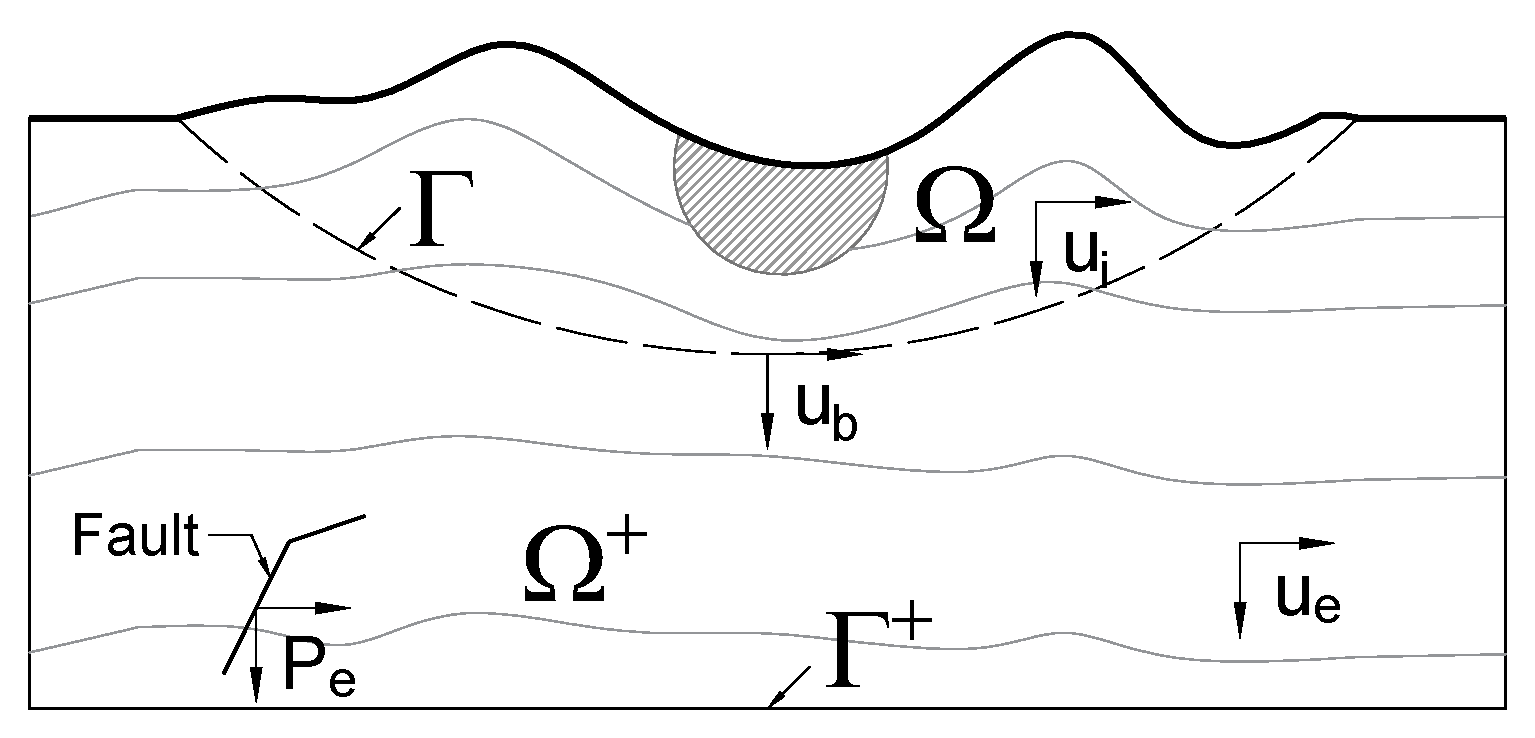
\includegraphics[width=3 in]{images/BIELAK0.pdf}}\\
\subfloat{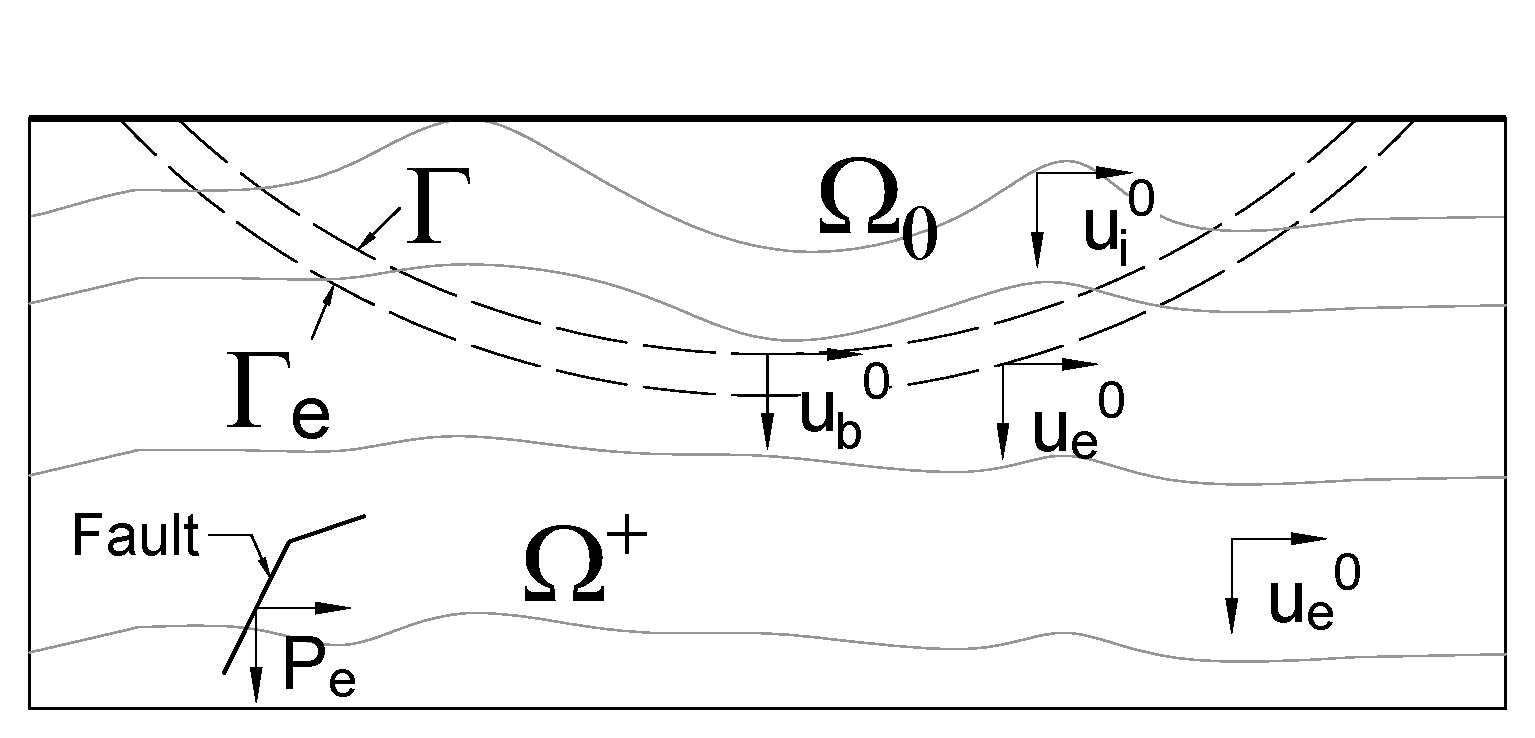
\includegraphics[width=3 in]{images/BIELAK1.pdf}}
\subfloat{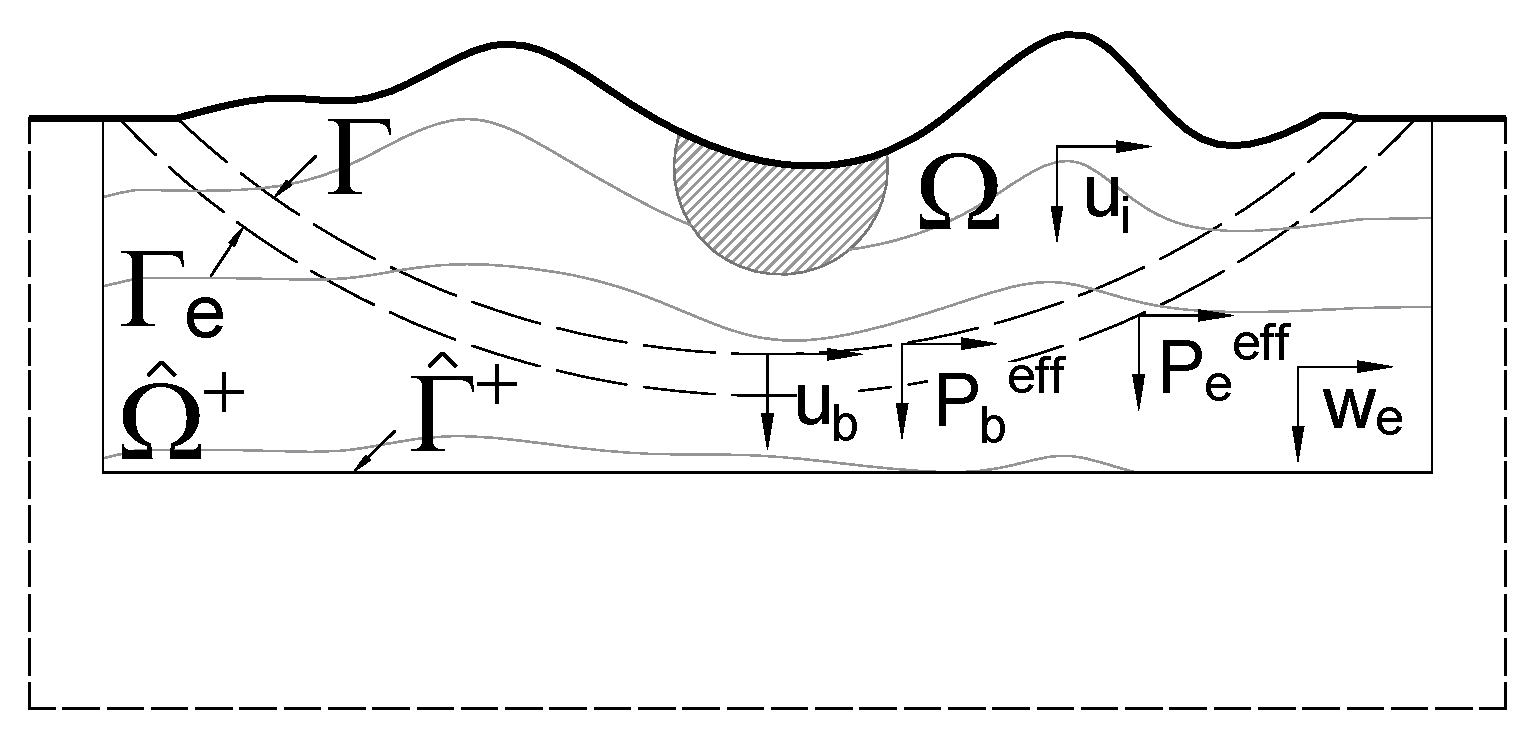
\includegraphics[width=3 in]{images/BIELAK2.pdf}}
\caption{Generalized partition of the total domain and its related fields in the original DRM algorithm. The first analysis step is conducted over the half-space with domain $\Omega^+ \cup \Omega_0$ (bottom left). The resulting motion is then applied as input excitation to the reduced domain $\hat{\Omega} ^+ \cup \Omega$ comprising only the localized feature (bottom right).}
\label{fig:bielak}
\end{figure}



In the original DRM method the effect of the seismic sources $P_e$ is transferred to the coupling surface $\Gamma$ using an auxiliary problem (or background structure) constructed after removing from the complete domain the scatterer $\Omega$ and replacing it by an arbitrary simplified domain $\Omega_0$ resulting in a generalized half-space $\Omega^+ \cup \Omega_0$ (as shown in the left part of \cref{fig:bielak}). This arbitrary domain is selected in such a way that it is easier to discretize than the original problem. The equations of motion for the domain $\Omega^+$ in the auxiliary problem under the action of the seismic sources $P_e$ yields a generalized free field motion $u^0$ governed by;


\begin{equation}
\left[ {\begin{array}{*{20}{c}}
{M_{bb}^{{\Omega ^ + }}}&{M_{be}^{{\Omega ^ + }}}\\
{M_{eb}^{{\Omega ^ + }}}&{M_{ee}^{{\Omega ^ + }}}
\end{array}} \right]\left\{ {\begin{array}{*{20}{c}}
{\ddot u_b^0}\\
{\ddot u_e^0}
\end{array}} \right\} + \left[ {\begin{array}{*{20}{c}}
{K_{bb}^{{\Omega ^ + }}}&{K_{be}^{{\Omega ^ + }}}\\
{K_{eb}^{{\Omega ^ + }}}&{K_{ee}^{{\Omega ^ + }}}
\end{array}} \right]\left\{ {\begin{array}{*{20}{c}}
{u_b^0}\\
{u_e^0}
\end{array}} \right\} = \left\{ {\begin{array}{*{20}{c}}
{ - P_b^0}\\
{{P_e}}
\end{array}} \right\}
\label{ffield}
\end{equation}

allowing to express the seismic sources like;


\begin{equation}
{P_e} = M_{eb}^{{\Omega ^ + }}\ddot u_b^0 + M_{ee}^{{\Omega ^ + }}\ddot u_e^0 + K_{eb}^{{\Omega ^ + }}u_b^0 + K_{ee}^{{\Omega ^ + }}u_e^0.
\label{source}
\end{equation}

The presence of the terms $M_{ee}^{{\Omega ^ + }}\ddot u_e^0$ and ${K_{ee}^{{\Omega ^ + }}u_e^0}$ in \cref{source} imply that the free field $u^0$ must be stored throughout the full domain $\Omega^+$. This inconvenient requirement is dealt with after writing the total field in the exterior part of $\Omega^+$ like a superposition of the free field motion $u_e^0$ and the relative (or scattered) motion $w_e$ as;

\begin{equation}
u_e=u_e^0+w_e
\label{relative}
\end{equation}

which yields;

\begin{equation}
\begin{array}{l}
\left[ {\begin{array}{*{20}{c}}
{M_{ii}^\Omega }&{M_{ib}^\Omega }&0\\
{M_{bi}^\Omega }&{M_{bb}^\Omega  + M_{bb}^{{\Omega ^ + }}}&{M_{be}^{{\Omega ^ + }}}\\
0&{M_{eb}^{{\Omega ^ + }}}&{M_{ee}^{{\Omega ^ + }}}
\end{array}} \right]\left\{ {\begin{array}{*{20}{c}}
{{{\ddot u}_i}}\\
{{{\ddot u}_b}}\\
{{{\ddot w}_e}}
\end{array}} \right\} + \left[ {\begin{array}{*{20}{c}}
{K_{ii}^\Omega }&{K_{ib}^\Omega }&0\\
{K_{bi}^\Omega }&{K_{bb}^\Omega  + K_{bb}^{{\Omega ^ + }}}&{K_{be}^{{\Omega ^ + }}}\\
0&{K_{eb}^{{\Omega ^ + }}}&{K_{ee}^{{\Omega ^ + }}}
\end{array}} \right]\left\{ {\begin{array}{*{20}{c}}
{{u_i}}\\
{{u_b}}\\
{{w_e}}
\end{array}} \right\}\\
 = \left\{ {\begin{array}{*{20}{c}}
0\\
{ - M_{be}^{{\Omega ^ + }}\ddot u_e^0 - K_{be}^{{\Omega ^ + }}u_e^0}\\
{{P_e} - M_{ee}^{{\Omega ^ + }}\ddot u_e^0 - K_{ee}^{{\Omega ^ + }}u_e^0}
\end{array}} \right\}
\end{array}
\label{iii-drm}
\end{equation}

After substituting for $P_e$ from \cref{source} into \cref{iii-drm} the equations of motion are written in terms of degrees of freedom over a single layer of finite elements in $\Omega^+$ adjacent to $\Gamma$. This strip of 1-element width lies between $\Gamma$ and its adjacent surface $\Gamma_e$ (see \cref{fig:bielak});

\begin{equation}
\begin{array}{l}
\left[ {\begin{array}{*{20}{c}}
{M_{ii}^\Omega }&{M_{ib}^\Omega }&0\\
{M_{bi}^\Omega }&{M_{bb}^\Omega  + M_{bb}^{{\Omega ^ + }}}&{M_{be}^{{\Omega ^ + }}}\\
0&{M_{eb}^{{\Omega ^ + }}}&{M_{ee}^{{\Omega ^ + }}}
\end{array}} \right]\left\{ {\begin{array}{*{20}{c}}
{{{\ddot u}_i}}\\
{{{\ddot u}_b}}\\
{{{\ddot w}_e}}
\end{array}} \right\} + \left[ {\begin{array}{*{20}{c}}
{K_{ii}^\Omega }&{K_{ib}^\Omega }&0\\
{K_{bi}^\Omega }&{K_{bb}^\Omega  + K_{bb}^{{\Omega ^ + }}}&{K_{be}^{{\Omega ^ + }}}\\
0&{K_{eb}^{{\Omega ^ + }}}&{K_{ee}^{{\Omega ^ + }}}
\end{array}} \right]\left\{ {\begin{array}{*{20}{c}}
{{u_i}}\\
{{u_b}}\\
{{w_e}}
\end{array}} \right\}\\
 = \left\{ {\begin{array}{*{20}{c}}
0\\
{ - M_{be}^{{\Omega ^ + }}\ddot u_e^0 - K_{be}^{{\Omega ^ + }}u_e^0}\\
{M_{eb}^{{\Omega ^ + }}\ddot u_b^0 + K_{eb}^{{\Omega ^ + }}u_b^0}
\end{array}} \right\}
\end{array}
\label{drm1}
\end{equation}

The actual domain reduction leading to the method in the formulation from \cite{bielak2003} is possible after noticing that all the waves in the exterior region $\Omega^+$ are outgoing. Since the primary interest is in the determination of the response for the local site (i.e., a microzone) this fact suggests that the size of $\Omega^+$ can be drastically reduced. This exterior reduced domain in the DRM algorithm is termed $\hat{\Omega}^+$.

The following points regarding the DRM formulation must be highlighted. First the equations of motion given in \cref{coupled} when written in terms of the free field motion reads:


\begin{equation}
\begin{array}{l}
\left[ {\begin{array}{*{20}{c}}
{M_{ii}^\Omega }&{M_{ib}^\Omega }&0\\
{M_{bi}^\Omega }&{M_{bb}^\Omega  + M_{bb}^{{\Omega ^ + }}}&{M_{be}^{{\Omega ^ + }}}\\
0&{M_{eb}^{{\Omega ^ + }}}&{M_{ee}^{{\Omega ^ + }}}
\end{array}} \right]\left\{ {\begin{array}{*{20}{c}}
{{{\ddot u}_i}}\\
{{{\ddot u}_b}}\\
{{{\ddot u}_e}}
\end{array}} \right\} + \left[ {\begin{array}{*{20}{c}}
{K_{ii}^\Omega }&{K_{ib}^\Omega }&0\\
{K_{bi}^\Omega }&{K_{bb}^\Omega  + K_{bb}^{{\Omega ^ + }}}&{K_{be}^{{\Omega ^ + }}}\\
0&{K_{eb}^{{\Omega ^ + }}}&{K_{ee}^{{\Omega ^ + }}}
\end{array}} \right]\left\{ {\begin{array}{*{20}{c}}
{{u_i}}\\
{{u_b}}\\
{{u_e}}
\end{array}} \right\}\\
 = \left\{ {\begin{array}{*{20}{c}}
0\\
0\\
{M_{eb}^{{\Omega ^ + }}\ddot u_b^0 + M_{ee}^{{\Omega ^ + }}\ddot u_e^0 + K_{eb}^{{\Omega ^ + }}u_b^0 + K_{ee}^{{\Omega ^ + }}u_e^0}
\end{array}} \right\}.
\end{array}
\label{i-drm}
\end{equation}

However complete transfer of the seismic sources $P_e$ to the coupling surface $\Gamma$ is only achieved after one eliminates from \cref{i-drm} the terms $M_{ee}^{{\Omega ^ + }}\ddot u_e^0$ and ${K_{ee}^{{\Omega ^ + }}u_e^0}$ which is accomplished by introducing the change of variables resulting after writing the total field in the exterior part of $\Omega^+$ in terms of the free-field and relative motion. For this change of variables to remain valid it is required that the reduced exterior domain $\hat{\Omega}^+$ retains the same material properties as the original exterior domain $\Omega^+$. The resulting DRM approach can be summarized in the following two-step algorithm:

\begin{itemize}
\item In step-I the complete seismic domain $\Omega \cup \Omega^+$, comprising the seismic source and microzones of soft material properties is replaced by a simpler domain $\Omega_0 \cup \Omega^+$ which results after removing all the surface topography and localized features.

\begin{figure}[H]
\centering
\subfloat{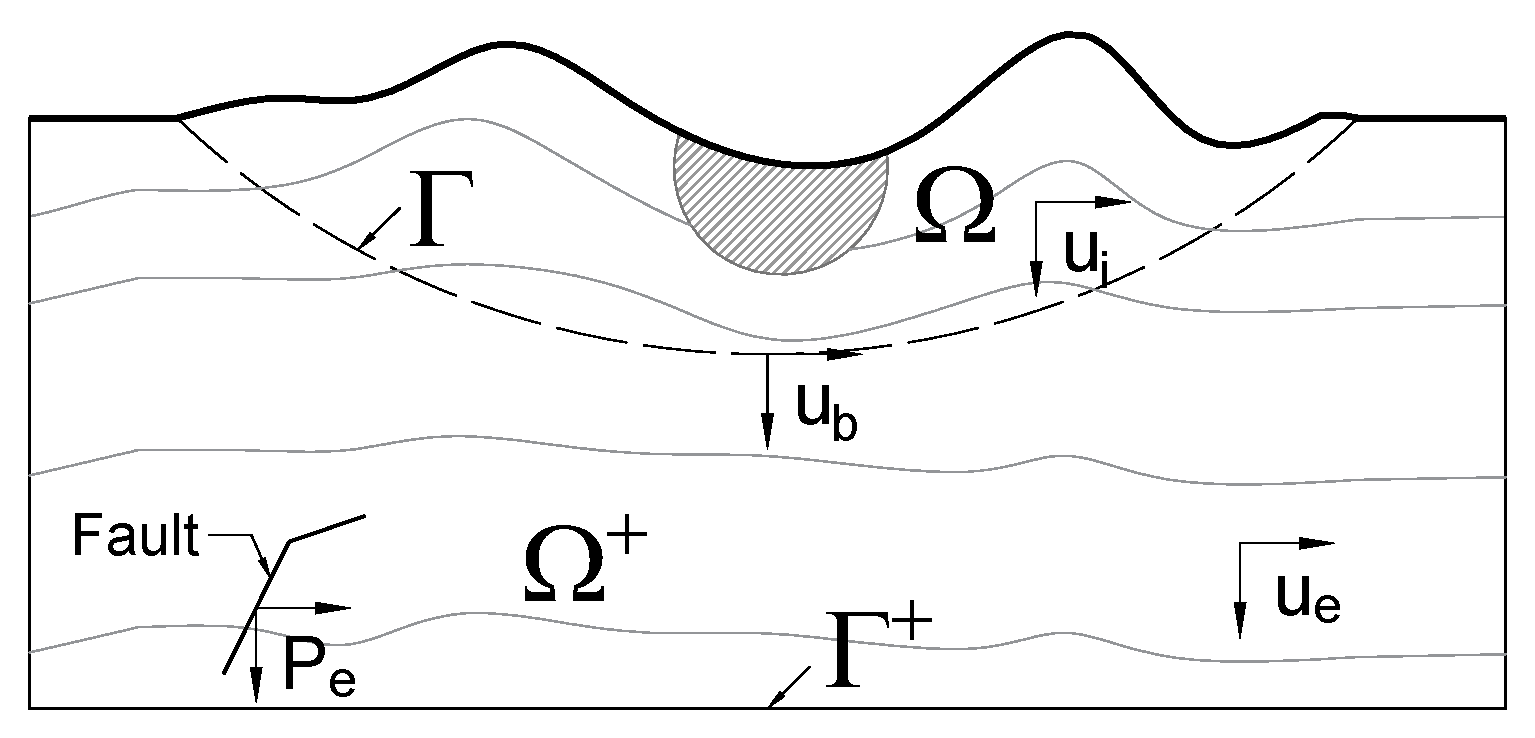
\includegraphics[width=3 in]{images/BIELAK0.pdf}}
\subfloat{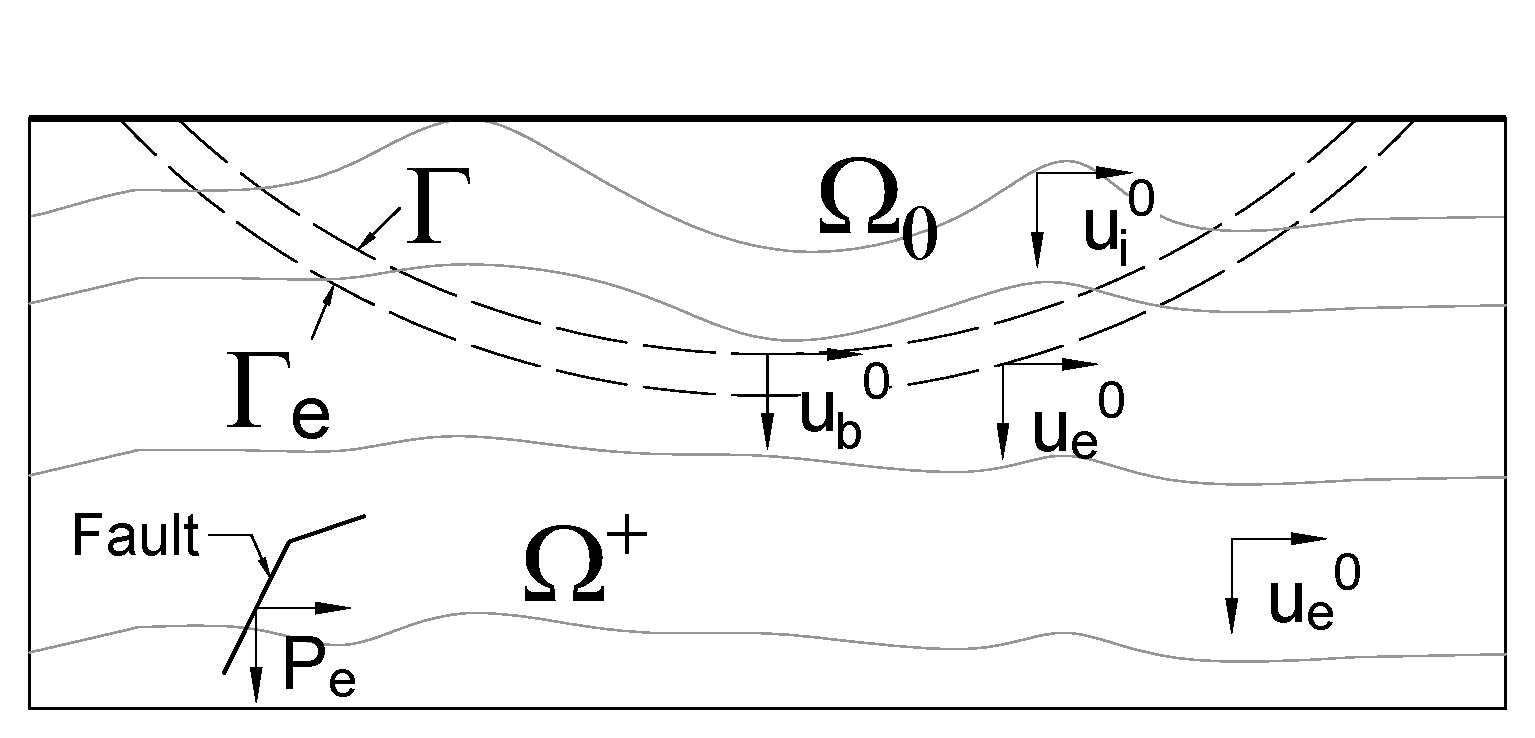
\includegraphics[width=3 in]{images/BIELAK1.pdf}}
\caption{In step I of the DRM algorithm the original domain $\Omega \cup \Omega^+$ (left) is replaced by a simpler domain $\Omega_0 \cup \Omega^+$ (right).}
\label{fig:SI}
\end{figure}

This simpler domain is analyzed, under the action of seismic sources $P_e$, in order to determine the free field response leading to effective loads located over a boundary adjacent to the local site given by;

\begin{eqnarray}
{P^{eff}} = \left\{ {\begin{array}{*{20}{c}}
0\\
{ - M_{be}^{{\Omega ^ + }}\ddot u_e^0 - K_{be}^{{\Omega ^ + }}u_e^0}\\
{M_{eb}^{{\Omega ^ + }}\ddot u_e^0 + K_{ee}^{{\Omega ^ + }}u_e^0}
\end{array}} \right\}.
\label{effective}
\end{eqnarray}


\item In step-II of the algorithm, ground response analysis is performed at desired microzones using as excitation the free-field motion extracted from the data base created during step-I. In the case of a plane wave analysis the calculation of the incoming motion through the solution of the FE-system specified in step-I is unnecessary as the field can be obtained analytically. This computation is performed automatically by {\bf WAVES} in the elemental subroutines used to define the elements along the strip (see \cref{fig:SII}).

\begin{figure}[H]
\centering
\subfloat{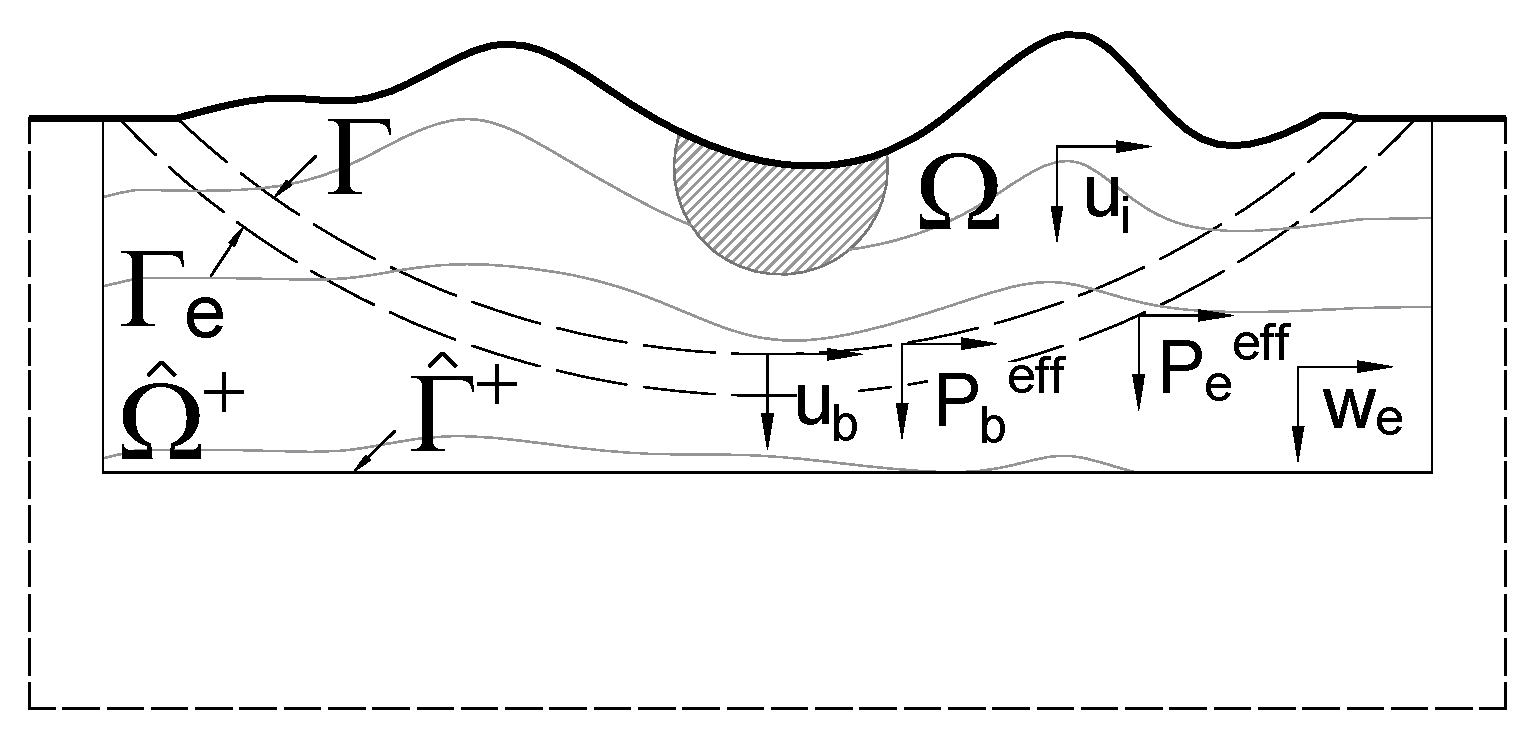
\includegraphics[width=3 in]{images/BIELAK2.pdf}}
\caption{Reduced domain subjected to the action of effective forces $P^{eff}$ and equivalent to the seismic sources.}
\label{fig:SII}
\end{figure}


The local model can take into account a highly detailed description of the small-scale topography. This local step can be performed using computing resources typically available at a consulting office and using an independent numerical technique.

\end{itemize}


A key aspect in the DRM technique is the fact that in the reduced domain $\hat{\Omega}^+ \cup \Omega$, the domain $\hat{\Omega}^+$ is of the same material properties as in the original $\Omega^+$ (right part of \cref{fig:bielak}). To reflect this fact the mass and stiffness coefficients pertaining to the domain $\hat{\Omega}^+$ have retained the superscript $\Omega^+$. 



\section{Explicit solution scheme}
Consider the discrete dynamic equilibrium equations at time $t$

\begin{equation}
M^{t}A+C^{t}V+K^{t}U=^{t}F
\label{equil}
\end{equation}

and where $M$, $C$, $K$ are the assembled mass, damping and stiffness matrices respectively while $^{t}A$, $^{t}V$, $^{t}U$ and  $^{t}F$ are the nodal accelerations, velocities, displacements and external loads vectors at time $t$. In {\bf WAVES} the external forces may be the result of particular point loads or effective forces consistent with a plan wave analysis.

In terms of nodal forces, \cref{equil} can be written like;

\begin{equation}
^{t}F^I+^{t}F^D+^{t}F^s=^{t}F
\label{force equil}
\end{equation}

where $^{t}F^I$, $^{t}F^D$ and $^{t}F^s$ are inertial, damping, elastic and external nodal forces respectively.

Expanding the acceleration and velocity terms at time $t$ in a consistent finite central differences scheme we have;

\begin{equation}
\begin{aligned}
^{t}A&=\dfrac{1}{\Delta t^2}\left(^{t-\Delta t}U-2^{t}U+^{t+\Delta t}U\right)\\
^{t}V&=\dfrac{1}{2\Delta t}\left(-^{t-\Delta t}U+^{t+\Delta t}U\right).
\end{aligned}
\label{finitediff}
\end{equation}

Consider now the trial states


\begin{equation}
\begin{aligned}
{}^t\hat A & = \frac{1}{{\Delta {t^2}}}\left( {{}^{t - \Delta t}U - 2{}^tU} \right)\\
{}^t\hat V & =  - \frac{1}{{2\Delta t}}{}^{t - \Delta t}U
\end{aligned}
\label{pred}
\end{equation}


which allows us to write \cref{finitediff} like;

\begin{equation}
\begin{aligned}
{}^tA & = {}^t\hat A + \frac{1}{{\Delta {t^2}}}{}^{t + \Delta t}U\\
{}^tV & = {}^t\hat V + \frac{1}{{2\Delta t}}{}^{t + \Delta t}U
\end{aligned}
\label{precorr}
\end{equation}

Notice that the terms ${}^t\hat A$ and ${}^t\hat V$ result after assuming that $^{t+\Delta t}U = 0$ in \cref{finitediff} thus they are commonly referred to as predictors. Notice also that after the displacements at $t+\Delta t$ have been found the corrected values of $^{t}A$ and $^{t}V$ can be obtained via \cref{precorr}. In this sense the terms $\frac{1}{{\Delta {t^2}}}{}^{t + \Delta t}U$ and $\frac{1}{{2\Delta t}}{}^{t + \Delta t}U$ play the role of correctors to the initial predictors. The resulting algorithm is commonly referred to, by obvious reasons, as a predictor-corrector scheme.

Using \cref{precorr} in \cref{equil} results in the following equation governing the displacements at time $t+\Delta t$;


\begin{equation}
\left(\dfrac{1}{\Delta t^2}M+\dfrac{1}{2\Delta t}C\right) ^{t+\Delta t}U=^{t}F-M{}^t\hat A - C{}^t\hat V - K{}^tU
\label{resequil}
\end{equation}

The dynamic finite element equilibrium equations given in \cref{resequil} can be written in the standard static form:

\[\hat K{}^{t + \Delta t}U = {}^t\hat F\]

after letting;

\[\hat K = \frac{1}{{\Delta {t^2}}}M + \frac{1}{{2\Delta t}}C\]

and

\[{}^t\hat F = {}^tF - M{}^t\hat A - C{}^t\hat V - K{}^tU\].



%%%%%

It is convenient, and physically appealing, to write \cref{resequil} in terms of forces like:


\begin{equation}
^{t+\Delta t}F^I+^{t+\Delta t}F^D=^{t}F-^t\hat {F}^I-^t\hat {F}^D-^{t}F^s
\label{force equil 2}
\end{equation}



\begin{itemize}
\item \Cref{force equil 2} is an equilibrium equation at time $t=t$ allowing to predict the displacements at time $t=t+\Delta t$ in terms of previously known values at times $t$ and $t=t-\Delta t$ as schematically shown in \cref{fig:time iteration}

\begin{figure}[h]
\centering
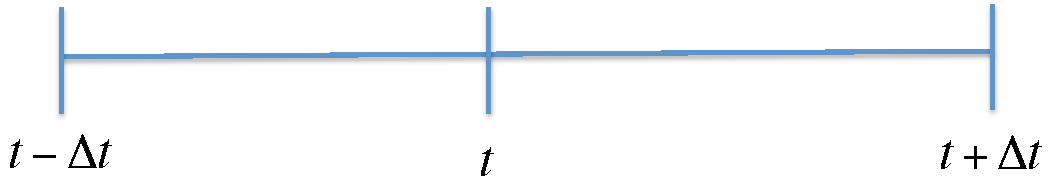
\includegraphics[width=12cm]{IMAGES/figure7_0.pdf}
\caption{Definition of the general iteration giving displacements at $t=t+\Delta t$ in terms of previously known values at times $t$ and $t=t-\Delta t$.}
\label{fig:time iteration}
\end{figure}

\item The equation is exact within the error introduced by the expansion used in \cref{finitediff}.



\item The first predicted solution is at $t=\Delta t$ which implies that we require data at $t=-\Delta t$ and at $t=0$ (i.e., initial conditions) as schematically shown in \cref{fig:initial time iteration}.

\begin{figure}[H]
\centering
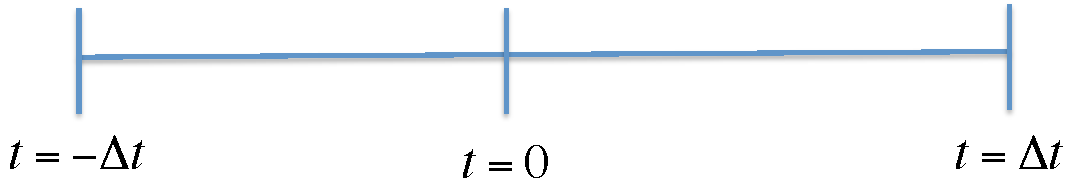
\includegraphics[width=12cm]{IMAGES/figure7_1.pdf}
\caption{Initial iteration predicting values at time $t=\Delta t$ in terms of the artifitial values at $t=-\Delta t$ and the initial conditions at  $t=0$.}
\label{fig:initial time iteration}
\end{figure}

\end{itemize}

\subsection*{Damping Assumptions}
The damping matrix $C$ appearing in \cref{resequil} is actually not assembled in the standard finite element sense but it is rather built from the mass and stiffness matrices. Moreover we can consider the following possibilities regarding damping.

\begin{itemize}
\item[(i)] Neglect damping (This is however inconvenient for finite domains) which gives:

\begin{equation}
^{t+\Delta t}F^I+^{t+\Delta t}F^D=^{t}F-^t\hat {F}^I-^{t}F^s
\label{Nodamping}
\end{equation}





\item[(ii)] Use Rayleigh Damping and retain the velocity expansion used in \eqref{finitediff}. That is;

\begin{equation}
C=\alpha M+\beta K
\end{equation}

then we have (in terms of forces);

\begin{equation}
(1+\beta \Delta t^2) ^{t+\Delta t}F^I+\dfrac{\alpha}{2\Delta t} ^{t+\Delta t}F^S=^{t}\hat{F}
\label{Rayleigh}
\end{equation}

where;

\[
^{t}\hat{F}=^{t}F-^t\hat {F}^I-^t\hat {F}^D-^{t}F^s
\]

Solution in equation \cref{Rayleigh} requires the full assembly and factorization of an effective stiffness matrix.



\item[(iii)] Use Rayleigh damping but modify the velocity expansion introduced in \cref{finitediff}. Using

\begin{equation}
^{t}V=\dfrac{1}{\Delta t}(^{t}U-^{t-\Delta t}U)
\label{velocity}
\end{equation}

yielding;

\begin{equation}
^{t+\Delta t}F^I=^{t}F-^t\hat {F}^I-^t\hat {F}^D-^{t}F^s
\end{equation}


where now the velocity predictor and corrector terms are defined like:

\[{}^t\hat V = \frac{1}{{\Delta t}}\left( {{}^tU - {}^{t - \Delta t}U} \right)\]

and 

\[{}^tV = \frac{1}{{2\Delta t}}\left( { - {}^{t - \Delta t}U + {}^{t + \Delta t}U} \right)\]

respectively, giving the equation:

\begin{equation}
^{t+\Delta t}F^I=^{t}F-^t\hat {F}^I-^{t}F^s-^t\hat {F}^D
\label{modvelocity}
\end{equation}

\end{itemize}

\subsection*{Algorithm implemented in {\bf WAVES} (damping assumption 3)}

Let us write \cref{modvelocity} like

\begin{equation}
^{j+1}F^I=^{j}F-^t\hat {F}^I-^{j}F^s-^j\hat {F}^D.
\label{modveliter}
\end{equation}

The first prediction corresponding to $t=\Delta t$ is given by;



\[{}^{\Delta t}{F^I} = {}^0F - {}^0{{\hat F}^I} - {}^0{{\hat F}^S} - {}^0{{\hat F}^D}\]

which results after applying \cref{modvelocity} at $t=0$ and where the term

\[{}^0{{\hat F}^D} = C\frac{1}{{\Delta t}}\left( {{}^0U - {}^{ - \Delta t}U} \right)\]

requires knowing the fictitious value $-^{\Delta t}U$. This last term can be computed after applying the central difference expansion at $t=0$ and solving for $-^{\Delta t}U$ giving;

\begin{equation}
^{-\Delta t}U=^{0}U-\Delta t ^{0}V+\dfrac{\Delta t^2}{2} {^{0}A}
\label{initialU}
\end{equation}

Finally using \cref{initialU} in \cref{modveliter} allows us to start up the algorithm. The general and initial iteration are schematized in \cref{fig:general iteration} and \cref{fig:initial iteration} respectively.

\begin{figure}[H]
\centering
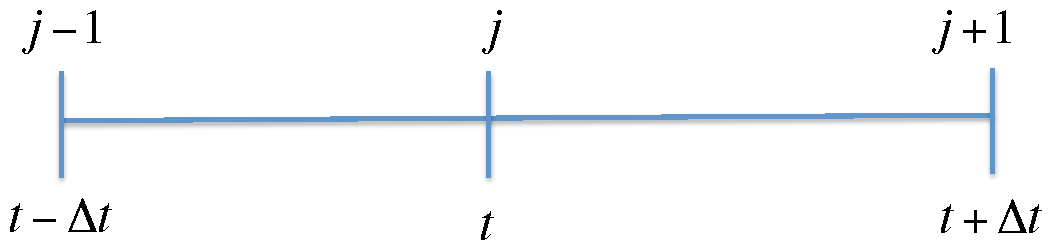
\includegraphics[width=12cm]{IMAGES/figure5.pdf}
\caption{Definition of the general iteration}
\label{fig:general iteration}
\end{figure}

\begin{figure}[H]
\centering
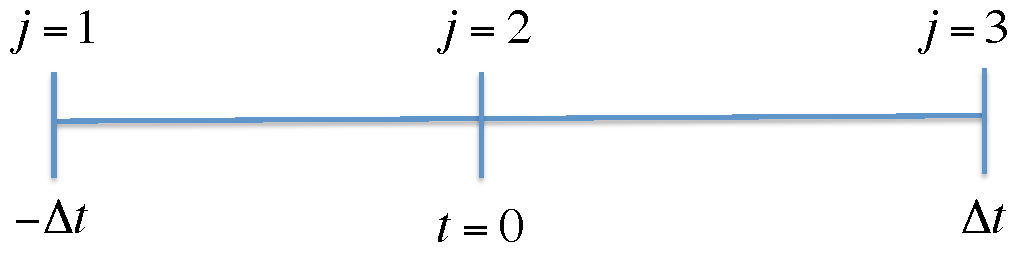
\includegraphics[width=12cm]{IMAGES/figure6.pdf}
\caption{Definition of the initial iteration}
\label{fig:initial iteration}
\end{figure}

%\subsubsection{Particulars}
%In what follows we concentrate on the algorithm corresponding to damping assumption 3 and in order to study some details we return to its standard displacements form. Writing \cref{modveliter} in terms of displacements and re-arranging terms gives us;


%\begin{equation}
%\dfrac{1}{\Delta t^2}M ^{t+\Delta t}U=^{t}F-(1+\dfrac{\beta}{\Delta t})K ^{t}U+(\dfrac{2}{\Delta t^2}-\dfrac{\alpha}{\Delta t})M ^{t}U-(\dfrac{1}{\Delta t^2} - \dfrac{\alpha}{\Delta t})M ^{t-\Delta t}U+(\dfrac{\beta}{\Delta t}) K ^{t-\Delta t}U.
%\label{disequil}
%\end{equation}
%
%Introduce the constants:
%
%
%\[
%\begin{aligned}
%a_1&=1+\dfrac{\beta}{\Delta t}\\
%a_2&=\dfrac{2}{\Delta t^2}-\dfrac{\alpha}{\Delta t}\\
%a_3&=\dfrac{1}{\Delta t^2} - \dfrac{\alpha}{\Delta t}\\
%a_4&=\dfrac{\beta}{\Delta t}
%\end{aligned}
%\]
% and write:
%
%\begin{equation}
%^{t+\Delta t}F^I=^{t}F-a_1K ^{t}U+a_2M ^{t}U-a_3M ^{t-\Delta t}U+a_4K ^{t-\Delta t}U
%\label{equliassum3}
%\end{equation}


\subsection{Decoupling}
The equilibrium equations discussed so far can be decoupled whenever the coefficient matrix is diagonal. As a result, the algorithm can proceed one degree of freedom at a time without the need for a complete assembly process and with large memory savings. Consider the particular case of damping assumption 3 and a lumped mass matrix. Writing  \cref{modveliter} for the $i$-th degree of freedom (i.e., $i$ is kept fixed ) results in:

\begin{equation}
\dfrac{1}{\Delta t^2}M_{ij} ^{t+ \Delta t}U_j=^{t}F_i-K_{ij} {^{t}U_j}-M_{ij} {^{t}\hat{A}_j}-C_{ij}{^{t}\hat{V}_j}
\label{equildecoupled1}
\end{equation}

Now, if the lumped mass matrix is written like;

\[
M_{ij}=m_I\delta_{ij}
\]

we have:


\begin{equation}
\dfrac{1}{\Delta t^2}m_I ^{t+ \Delta t}U_i=^{t}F_i-K_{ij} {^{t}U_j}-m_{I} {^{t}\hat{A}_i}-C_{ij}{^{t}\hat{V}_j}
\label{equildecoupled2}
\end{equation}


producing the following recursive equation;

\begin{equation}
^{t+\Delta t} F_i^I=^{t}F_i-^{t} \hat{F}^S_i-{^{t}\hat{F}_i}^I-{^{t}\hat{F}_i}^D.
\label{forces3}
\end{equation}


To initialize the algorithm we apply the FDs equations at $t=0$ leading to:

\[
\dfrac{1}{\Delta t^2}m_I ^{\Delta t}U_i=^{0}F_i-K_{ij} {^{0}U}_j-m_I {^{0}\hat{A}}_i-C_{ij} {^{0}\hat{V}}_i.
\]

In the above we require:

\[
^{0}\hat{V} = \frac{1}{{\Delta t}}\left( {{}^0{U_i} - {}^{ - \Delta t}{U_i}} \right)
\]

which at the same time implies prior knowledge of the artificial term  $^{-\Delta t} U_i$. This can be obtained from \eqref{initialU} as follows:

\begin{equation}
^{-\Delta t}U_i=^{0}U_i-\Delta t {^{0}V}_i+\dfrac{\Delta t^2}{2} {^{0}A}_i.
\label{initialU2}
\end{equation}

The initial acceleration is obtained after assuming homogeneous ICs;

\[
m_{I} {^{0}A}_i+C_{ij} {^{0}V}_j +K_{ij} {^{0}U}_j=^{0}F_i
\]

therefore

\[m_{I} ^{0}A_i=\dfrac{^{0}F_i}{m_I}\]

and

\[^{-\Delta t} U_i=\dfrac{\Delta t^2}{2m_I}{^{0}F}_i.
\]



Moreover, neglecting the damping effects on the prediction of $^{\Delta t}U_i$ yields;

\[
^{\Delta t} U_i=\dfrac{\Delta t^2}{2m_I}{^{0}F}_i
\]

%\subsubsection*{Algorithms}

%\begin{algorithm}[H]
%\SetAlgoLined
%\KwData{Values at $t=0$, Geometry, Material Parameters}
%\KwResult{Displacements, Velocity and Acceleration at any time $t=t$ }
%Compute predictors ${}^t\hat A$, ${}^t\hat V$, ${}^t\hat U$\\
%Assemble  $\hat K$, ${}^t\hat F$\\
%Solve $\hat K{}^{t + \Delta t}U = {}^t\hat P$\\
%Perform Corrections ${}^tA \leftarrow {}^t\hat A + \frac{1}{{2\Delta {t^2}}}{}^{t + \Delta t}U$ and ${}^tV \leftarrow {}^t\hat V + \frac{1}{{2\Delta t}}{}^{t + \Delta t}U$
%\caption{Explicit algorithm}
%\end{algorithm}
%
%\newpage
%
%\begin{algorithm}[H]
%\SetAlgoLined
%\KwData{Time span, Geometry, Material Parameters}
%\KwResult{Displacements, Velocity and Acceleration time histories }
%Compute $^{t+\Delta t} F_i^I$\\
%Solve for $^{t+\Delta t}U_i=\left(\dfrac{\Delta t^2}{m_I}\right) ^{t+\Delta t}F_{i}^I$\\
%Update $^{t}V_i$, $^{t}A_i$
%\caption{Summarized Algorithm}
%\end{algorithm}
%
%\newpage

\begin{algorithm}[H]
 \SetAlgoLined
 \KwData{Time span, Geometry, Material Parameters}
 \KwResult{Displacements, Velocity and Acceleration time histories }
 Initialize solution vectors ($j=1$ corresponds to ICs: $0$ superscript indicates $t=0$)\;
 $^{0}U_i\longleftrightarrow ^{j = 1}U_i=0$, $^{0}V_i=0$, $^{j = 1}A_i=\dfrac{^{1}R_i}{m_I}$ \;
 Select $\Delta t$ and damping coefficients $\alpha$, $\beta$\;
 Fix 1-st predicted value (let $j=2$)\;
 \[
^{\Delta t} U_i \longleftarrow \dfrac{\Delta t^2}{2m_I} {^{0}F}_i\longleftrightarrow \left[^{j = 2}U_i \longleftarrow\dfrac{\Delta t^2}{2m_I} {^{j = 1}F}_i \right]
 \]
Time Integration Phase\;
\While{$j \leq N$}{
\[
\begin{aligned}
Predictors\\
{}^j{{\hat A}_i}\leftarrow&\frac{1}{{\Delta {t^2}}}\left( {{}^{j - 1}{U_i} - 2{}^j{U_i}} \right)\\
{}^j{{\hat V}_i} \leftarrow&\frac{1}{{\Delta t}}\left( {{}^j{U_i} - {}^{j - 1}{U_i}} \right)\\
^{j+1}F^I_i\longleftarrow& ^{j}F_i-K_{ij} {^{j}U}_j-m_I {^{j}\hat{A}}_j-C_{ij} {^{j-1}\hat{V} }_j\\
Solve\\
 ^{j+1}U_i\longleftarrow&\dfrac{\Delta t^2}{m_I} {^{j+1}F_i}^I\\
 Correctors\\
 {}^j{A_i}\leftarrow& {}^j{{\hat A}_i} + \frac{1}{{\Delta {t^2}}}{}^{j + 1}{U_i}\\
 {}^j{V_i} \leftarrow& {}^j{{\hat V}_i} + \frac{1}{{2\Delta t}}{}^{j + 1}{U_i}\\
 j\longleftarrow&j+1
\end{aligned}
\]
}
\caption{Full Algorithm}
\end{algorithm}



\subsection*{Program structure}
In the explicit integration scheme the solution corresponding to the $i$-th degree of freedom at time $t + \Delta t$ is found from \cref{predictive}:

\begin{equation}
^{j+1}U_i\longleftarrow \left( \dfrac{\Delta t^2}{m_I}\right) {^{j+1}F^I}_i
\label{predictive}
\end{equation}

where $m_I$ is the total mass associated to the $i$-th degree of freedom and $^{j+1}F^I_i$ is the total force considering the contribution from the external, elastic, inertial and damping terms at times $t$ and $t - \Delta t$. This force is given by \cref{mainforce}:

\begin{equation}
^{j+1}F^I_i\longleftarrow ^{j}F_i-K_{ij} {^{j}U}_j-m_I {^{j} \hat{A}}_i- C_{ij} {^{j} \hat{V} }_j.
\label{mainforce}
\end{equation}


Accordingly, in the uncoupled explicit finite element formulation the equation solving process proceeds one degree of freedom at a time. This implies a different assembly process to the one used in an implicit algorithm where a formal coefficient matrix is assembled and inverted. Now the mass, damping and stiffness elemental matrices are used to obtain effective nodal forces at each degree of freedom. In summary the mesh is not covered in an element by element basis, but in a node by node basis. In the following algorithm we discuss this nodal assembly process where in order to solve the displacement at a given degree of freedom prior knowledge of the elements contributing to the given node is necessary.

In particular in {\bf WAVES} the total mass $m_I$  and the total force $^{j+1}F^I_i$ is built after considering the contribution from the different elements connected to the node. This nodal assembly process is schematized in \cref{fig:ensambla} in which 4 bi-lineal elements are connected by a central node.


\begin{figure}[H]
\centering
\subfloat{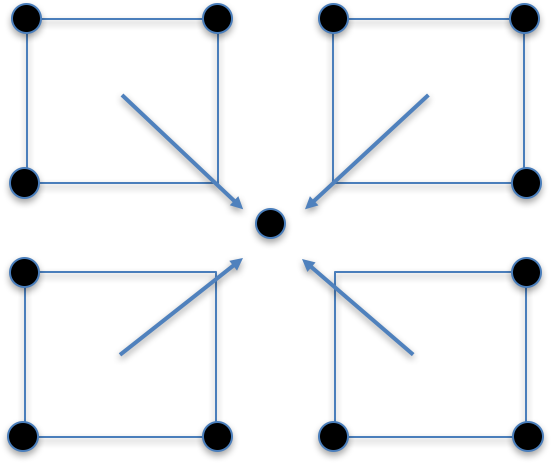
\includegraphics[width=7.0 cm]{img/assembly}}
\caption{Nodal assembly}
\label{fig:ensambla}
\end{figure}



\vspace{1.0 cm}

The nodal assembly is described in the following algorithm:

\vspace{1.0 cm}

\begin{algorithm}[H]
 \SetAlgoLined
 \KwData{Number of elements connected to the node}
 \KwResult{Total mass and force contribution }
\For {$i \longleftarrow 1$ to $Numnp$}{
$k \longleftarrow NIEL_i$\\
\For {$j \longleftarrow 1$ to $k$}{
Retrieve element parameters\\
Compute predictors\\
Compute element contribution ({\bf UEL.for})\\
Assembly element contribution into the force vector $^{j+1}F^I_i$\\

}
Solve for the current d.o.f\\
Perform corrections.

}

\caption{Nodal assembly}
\end{algorithm}

\vspace{1.0 cm}

The subroutine {\bf UEL.for} in the algorithm computes the contribution from the current element to the degree of freedom being solved. The library of available elements in the code corresponds precisely to a set of {\bf UELs} subroutines. Additional elements can be easily implemented and added to the code by just coding new {\bf UEL} subroutines as will be specified later.



\subsection*{Elements}
The following elements are currently available in {\bf WAVES} : 
\begin{verbatim}
UELEXP8: 8-noded 2D quad element.
UELEXP4: 4-noded 2D quad element. 
UELEXP9: 9-noded 2D quad element.
UELEXP6: 6-noded 2D triangular element.
UEL8INCOT: 8-noded 2D quad element with plane-wave incoming effective DRM forces.
UEL9INCOT: 9-noded 2D quad element with plane-wave incoming effective DRM forces.
UELEDASH3: 3-noded 2D Lysmer and Kuhlemeyer absorbing boundary.
UELDASHINC: 3-noded 2D transmitting boundary.
UEL3DEXP8: 8-noded bilineal 3D tetrahedarl elment.
\end{verbatim}

\subsection{Adding elements}
User element subroutines may be added to the code by implementing a {\bf UEL} subroutine with the following interface.


\begin{verbatim}
      SUBROUTINE UELXXX(RHS,ANMASS,NDOFEL,PROPS,NPROPS,IPROPS,NIPROPS,
     1                   AWAVE,IWAVE,COORDS,MCRD,NNODE,U,DU,V,A,JELEM,
     2                   DT,KINC,NINCR)
     
      IMPLICIT REAL*8(A-H,O-Z)

      PARAMETER (ZERO=0.D0,HALF=0.5D0,ONE=1.D0,NTENS=4,TWO=2.D0,NGPTS=9,
     1           THREE=3.D0, NDI=3)

C     Parameter arrays from UEL.f

      DIMENSION RHS(NDOFEL),ANMASS(NDOFEL),PROPS(NPROPS),
     1          IPROPS(NIPROPS),AWAVE(5),COORDS(MCRD,NNODE),U(NDOFEL),
     2          DU(NDOFEL),V(NDOFEL),A(NDOFEL),AMATRX(NDOFEL,NDOFEL),
     3          AMASS(NDOFEL,NDOFEL),CDMAT(NDOFEL,NDOFEL),UP(NDOFEL),
     4          DDSDDE(NTENS,NTENS),B(NTENS,NDOFEL),BT(NDOFEL,NTENS),
     5          FRST2(NDOFEL,NDOFEL),FRST1(NDOFEL,NDOFEL),XP(2,NGPTS),
     6          XW(NGPTS),AUX1(NTENS,NDOFEL)



      RETURN
\end{verbatim}
The subroutine must return the following parameters to the main program:

\begin{itemize}
\item[•] RHS: Contribution from the current element to the $i$-th degree of freedom total external force as given by \cref{mainforce}.
\item[•] ANMASS: Contribution from the current element to the $i$-th degree of freedom total mass. 
\end{itemize}

On the other hand the input parameters are defined as follows:

\begin{itemize}
\item[•] NDOFEL: Total number of degrees of freedom of the elemnt.
\item[•] PROPS: Array containing the real material properties needed to compute the forces in the current element.
\item[•] NPROPS: Dimension of the PROPS array.
\item[•] IPROPS: Array containing the integer material properties needed to compute the forces in the current element. This arrays is mainly used in the definition of incoming elements in order to specify which face of the element is in direct contact with the scatterer.
\item[•] NIPROPS: Dimension of the IPROPS array.
\item[•] AWAVE: Plan wave parameters.
\item[•] IWAVE: Dimension of the AWAVE array.
\item[•] COORDS: Array with the nodal coordinates of the element.
\item[•] MCRD: Parameter defining the dimensionality of the problem.
\item[•] NNODE: Total number of nodes in the element.
\item[•] U: Nodal displacements at time $t$.
\item[•] DU: Displacement increment defined as $\Delta U = {}^tU - {}^{t - \Delta t}U$.
\item[•] V: Trial velocity defined as ${}^t\hat V =  - \frac{1}{{2\Delta t}}{}^{t - \Delta t}U$ .
\item[•] A: Trial acceleration defined as ${}^t\hat A  = \frac{1}{{\Delta {t^2}}}\left( {{}^{t - \Delta t}U - 2{}^tU} \right)$ .
\item[•] JELEM: Current element identifier.
\item[•] DT: Size of the time step.
\item[•] KINC: Current increment number.
\item[•] NINCR: Total number of increments.
\end{itemize}


\section{Modeling a wave propagation problem with WAVES}

In {\bf WAVES} a finite element model is defined through an input data file with extension {\bf .inp} as described in the file named {\bf template.inp}. The file contains the following general data blocks.

\begin{verbatim}
PROBLEM DEFINITION BLOCK
NODAL DEFINITION BLOCK
MATERIAL DEFINITION BLOCK
WAVE DEFINITION BLOCK
ELEMENTS DEFINITION BLOCK
POINT LOADS DEFINITION BLOCK
NODAL OUTPUT DEFINITION BLOCK
\end{verbatim}

A template file is provided with the code. The structure of the input data file is explained in the last section of this document.
\subsection*{Creating a model with Gmesh}
Although input data files for simple models can be created manually the process becomes cumbersome in large problems. In this section we describe how to define a model using the third party software {\bf Gmesh}. On the other hand, although the code can be used to solve virtually any dynamic loading problem, in the following example we focus in a plane wave analysis typically found in earthquake engineering. 

The creation of a {\bf WAVES} model in {\bf Gmesh} involves a three-step procedure:

\begin{itemize}
\item[(i)  ]  Definition of the model geometry through a {\bf Gmsh} {\bf *.geo} file.
\item[(ii) ]  Definition of the finite element mesh through a {\bf Gmsh}  {\bf *.msh} file.
\item[(iii)]  Definition of the input data file {\bf *.inp} using the python module {\bf meshio.py}.
\end{itemize}

\subsubsection*{Problem definition}
All the plane wave propagation problems in {\bf WAVES} can be defined starting from the fundamental geometry shown in \cref{fig:plantilla} given by an open rectangular box. This fundamental geometry represents a half-space or baserock used for the application of the plane incident waves. A plane wave scattering model can subsequently be created through the addition of a generalized geometry inside the rectangular box. The figure shows the pre-defined physical lines and surfaces as required by Gmsh and used later during the generation of the input file. The model is ahown upsidedown as originally created in Gmsh in order to preserve the typical wave propagation convention of having the $y$-axis pointing towards the interior of the half-space. \Cref{fig:modelo canon} shows the model corresponding to a scatterer conformed by triangular canyon. In terms of Gmsh entities the scatterer is conformed by the addition of the physical surface $12000$ and the lines $22$ through $25$ configuring the canyon.
  

\begin{figure}[H]
\centering
\subfloat{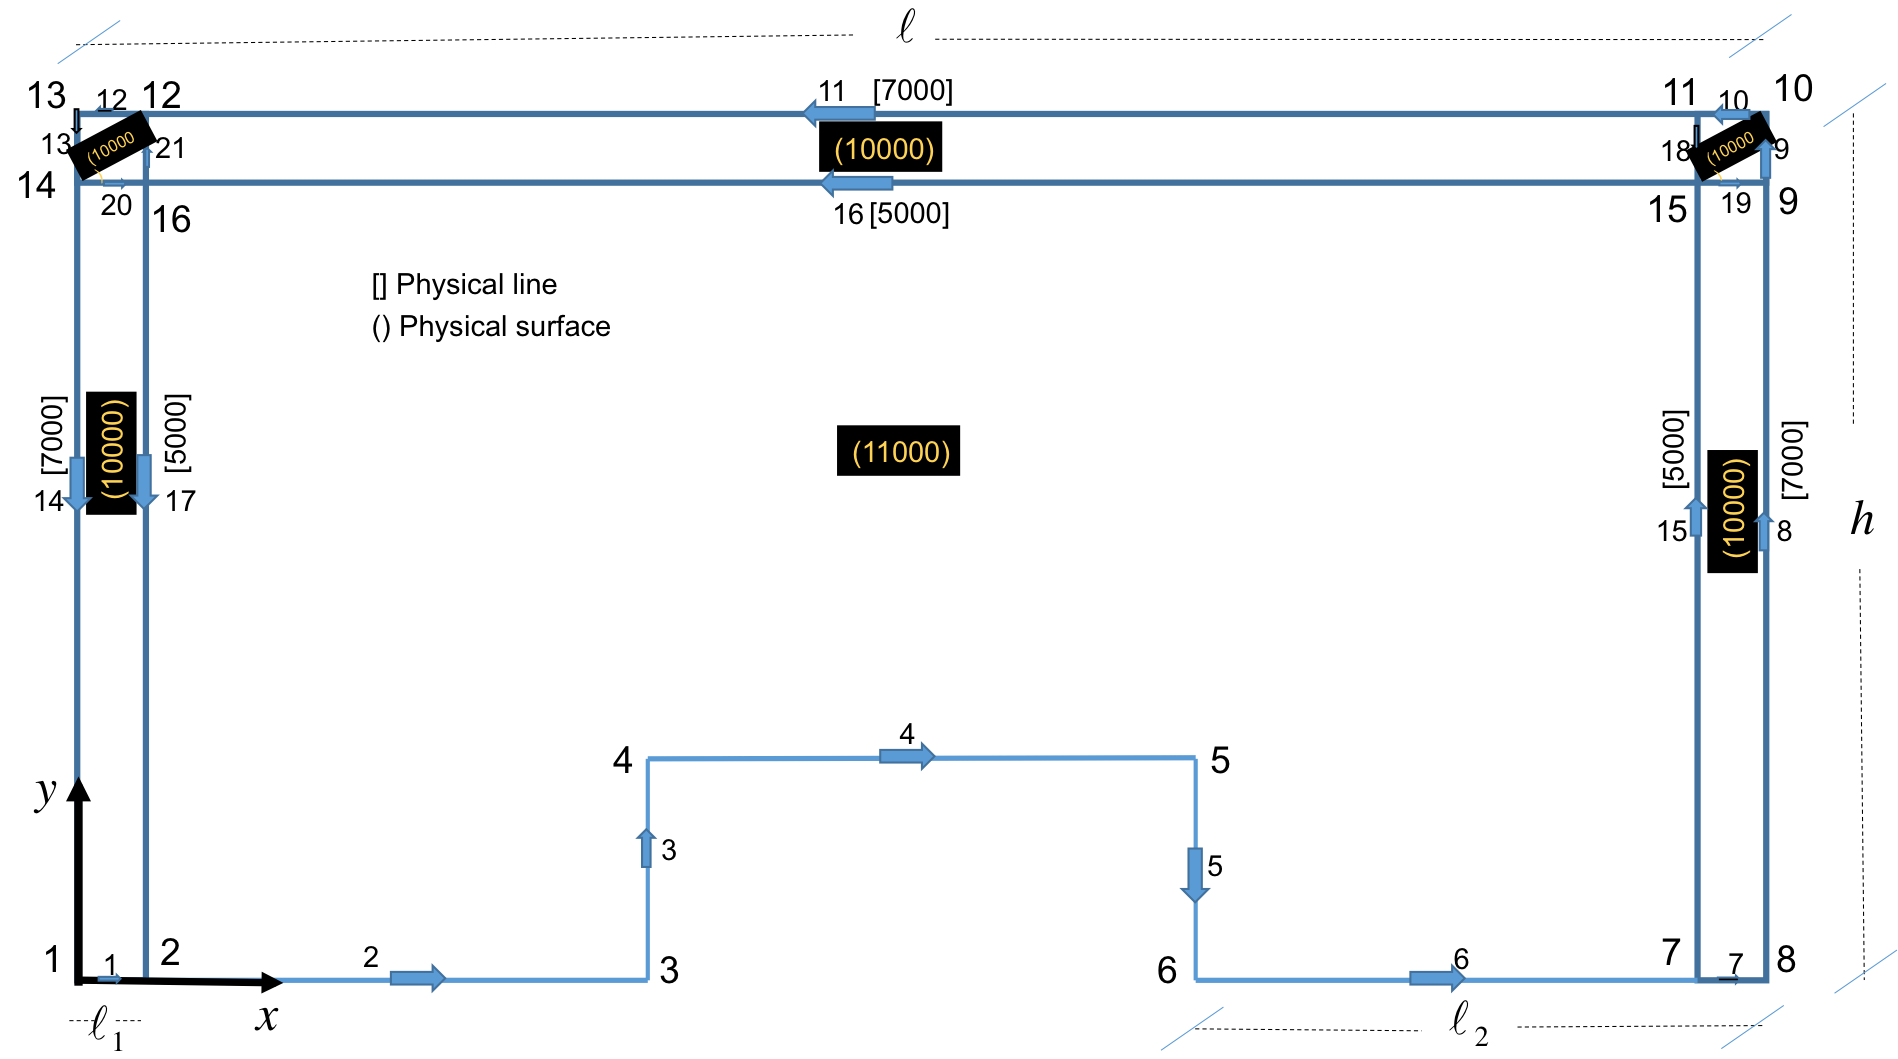
\includegraphics[width=16 cm]{img/plantilla04}}
\caption{Geometry of the general template conformed by a rectangular box used to represent the half-space.}
\label{fig:plantilla}
\end{figure}


\begin{figure}[H]
\centering
\subfloat{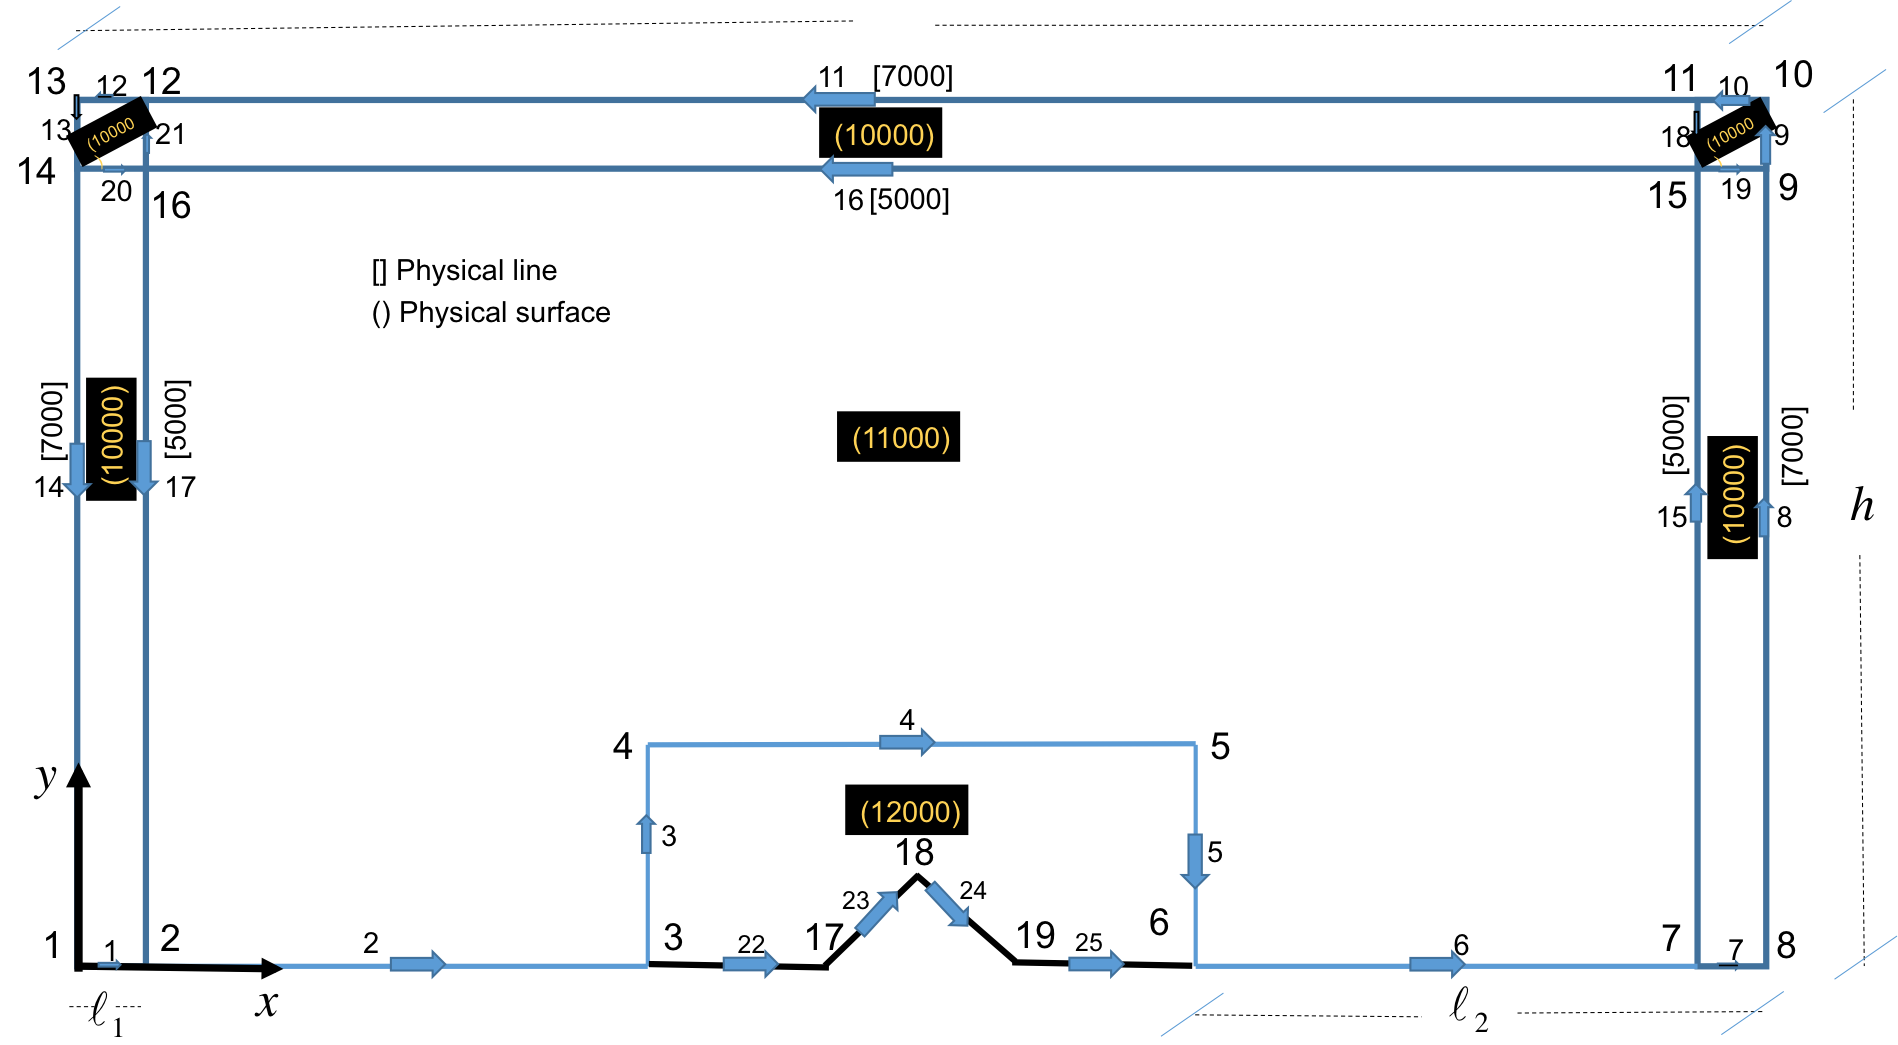
\includegraphics[width=16 cm]{img/canion2}}
\caption{Particular scatterer in the form of a V-shaped canyon added to the rectangular box.}
\label{fig:modelo canon}
\end{figure}

\subsubsection*{Meshing the model}
To conduct the wave propagation analysis using {\bf WAVES} the {\bf Gmsh} model must be converted into the {\bf .inp} data file. This reading and re-writing process is achieved using the Python module {\bf meshio} which directly reads the {\bf Gmsh} file into dictionaries which are later processed by problem-dependent python scripts. The conversion of a mesh into a {\bf WAVES} input file involves the generation of arrays storing the nodal and elementary data for the different parts of the model. A {\bf Gmsh} model is converted into a {\bf WAVES} model after processing the nodal data and each physical surface and physical line of the finite element model. This process is summarized as follows:

\begin{enumerate}
\item[•] Reading the {\bf Gmsh} data files using meshio.
\item[•] Storing the nodal data in a nodal array written in {\bf WAVES} format.
\item[•] Process each physical surface of the model and generate elementary arrays in {\bf WAVES} format.
\item[•] Process the physical line modeling the absorbing boundary condition and generate an additional elementary array.
\item[•] If any process additional physical lines to impose point loads and point loads array.
\item[•] Write all the arrays into a single {\bf WAVES} file. 
\end{enumerate}

These steps can be conducted using simple subroutines from the module mesh\_waves.py available in the folder {\bf MODELS$>$MESHER}. Each one of these subroutines is described next.

\subsubsection*{Nodal writer}
\begin{verbatim}
def node_writer(points , point_data):
    """
    Writes down the nodal data as required by WAVES.
        INPUT PARAMTERS:
    ---------------
        points and point_data: Are the dictionaries creatd by meshio.
    OUTPUT PARAMTERS:
    ----------------
        nodes_array : Integer array with the nodal data according to WAVES.
    """
\end{verbatim}
Takes as input parameters the dictionaries {\bf points} and {\bf point\_data} storing the nodal coordinates and nodal identifiers of nodal sets associated to physical entities. The subroutine returns as output parameter the array {\bf nodes\_array} ready to be written into the {\bf WAVES} input file.

\subsubsection*{Element writer}
Process each physical surface containing elements of the same type and of the same material profile. The subroutine takes as input parameters the dictionaries {\bf cells} and {\bf cell\_data} and the name of the physical surface where they belong. Upon execution the subroutine returns the number of elements contained in the set and an array with the elemental data written in {\bf WAVES} format.  The subroutine must be called one per each physical surface declared in the model. In order to keep a consecutive count in the number of elements the subroutine uses input and output parameters {\bf nini} and {\bf nf}. The former initializes the element count and the latter indicates the last element number on the set. When the subroutine is used to process consecutive physical surfaces the parameter {\bf nini} must be initialized with the last computed value of {\bf nf}. 

\begin{verbatim}
def ele_writer(cells , cell_data , ele_tag , phy_sur , ele_type , mat_tag , ndof ,
                       nnode , nini):
    """
    Extracts a subset of elements from a complete mesh according to the
    physical surface phy_sur and writes down the proper fields into an
    elements array.
    INPUT PARAMTERS:
    ---------------
        cell and cell_data: Are the dictionaries creatd by meshio.
        ele_tag : String defining the element type according to meshio 
        (e.g., quad9 , line3, etc).
        phy_sur : Integer defining the physical surface for the subset.
        ele_type: Integer defining the element type according to WAVES.
        mat_tag : Integer defining the material profile for the subset.
        ndof    : Integer defining the number of degrees of freedom for the elements.
        nnode   : Integer defining the number of nodes for the element.
        nini   : Integer defining the element id for the first element in the set.
    OUTPUT PARAMTERS:
    ----------------
        nf        : Integer defining the element id for the last element in the set
        els_array : Integer array with the elemental data according to WAVES.
    """
\end{verbatim}


\subsubsection*{Face recognition subroutine}
This subroutine is a special version of the element writer subroutine used to process the incoming elements containing the strip where the incident plane wave is applied in the form of effective forces through stiffness terms. In order to compute the effective loads these elements require specification of the normal vector of the element face in direct contact with the scatterer. The subroutine recognizes the corresponding element face by identifying the element nodes in contact with a specified physical line defining the halfspace-scatterer interface. The material profiles with identifiers $1$ through $4$ will then have an intger material property corresponding to the possible $4$ element faces. Accordingly material profile 4 in the input data file will be assigned to all the incoming elements with face number $4$ in contact with the scatterer-half-space physical line.


\begin{verbatim}
def face_recognition(cells , cell_data , phy_sur , phy_lin , nini):
    """
    For the incoming elements required to create a plane wave
    this function extracts the set according to the physical 
    surface and identifies the element face in contact with
    th scatterer.
    INPUT PARAMTERS:
    ---------------
        cell and cell_data: Are the dictionaries creatd by meshio
        phy_sur: Integer defining the physical surface for the strip.
        phy_lin: Integer defining the physical line for the strip-scatterer interface
        nini   : Integer defining the element id for the first element in the set.
    OUTPUT PARAMTERS:
    ----------------
        nf        : Integer defining the element id for the last element in the set
        els1_array: Integer array with the elemental data according to WAVES.
    """
\end{verbatim}

\subsubsection*{Absorbing boundary writer subroutine}
The Lysmer and Khulemeyer absorbing boundaries are specified in terms of a physical line in {\bf Gmsh}. The absorbing boundary writer subroutine identifies which line elements out of the {\bf cell\_data} dictionary belong to this physical line and subsequently write the specific element data in {\bf WAVES} format.

 
\begin{verbatim}
def boundary_writer(cells , cell_data , phy_lin , mat_tag , nini ):
    """
    Extracts a subset of line elements from a complete mesh and corresponding
    to Lysmer absorbing  boundaries. The elements are identified according to
    the physical line phy_lin.
    INPUT PARAMTERS:
    ---------------
        cell and cell_data: Are the dictionaries created by meshio.
        ele_tag : String defining the element type according to meshio
        (e.g., quad9 , line3, etc).
        phy_lin: Integer defining thw physical line for the strp-scatterer
        interface.
        mat_tag : Integer defining the material profile for the subset.
        nini   : Integer defining the element id for the first element in the set.
    OUTPUT PARAMTERS:
    ----------------
        nf        : Integer defining the element id for the last element in the set
        els_array : Integer array with the elemental data according to WAVES.
    """
\end{verbatim}  
  
\section*{Example: Creating the model for the generalized template}
Here we illustrate how to create a {\bf WAVES} model for the generalized template shown again in \cref{fig:plantilla2}. In the {\bf template.geo} file in {\bf Gmsh} the model has been divided into physical surfaces and physical lines identifying the different parts of the domain.

\begin{figure}[H]
\centering
\subfloat{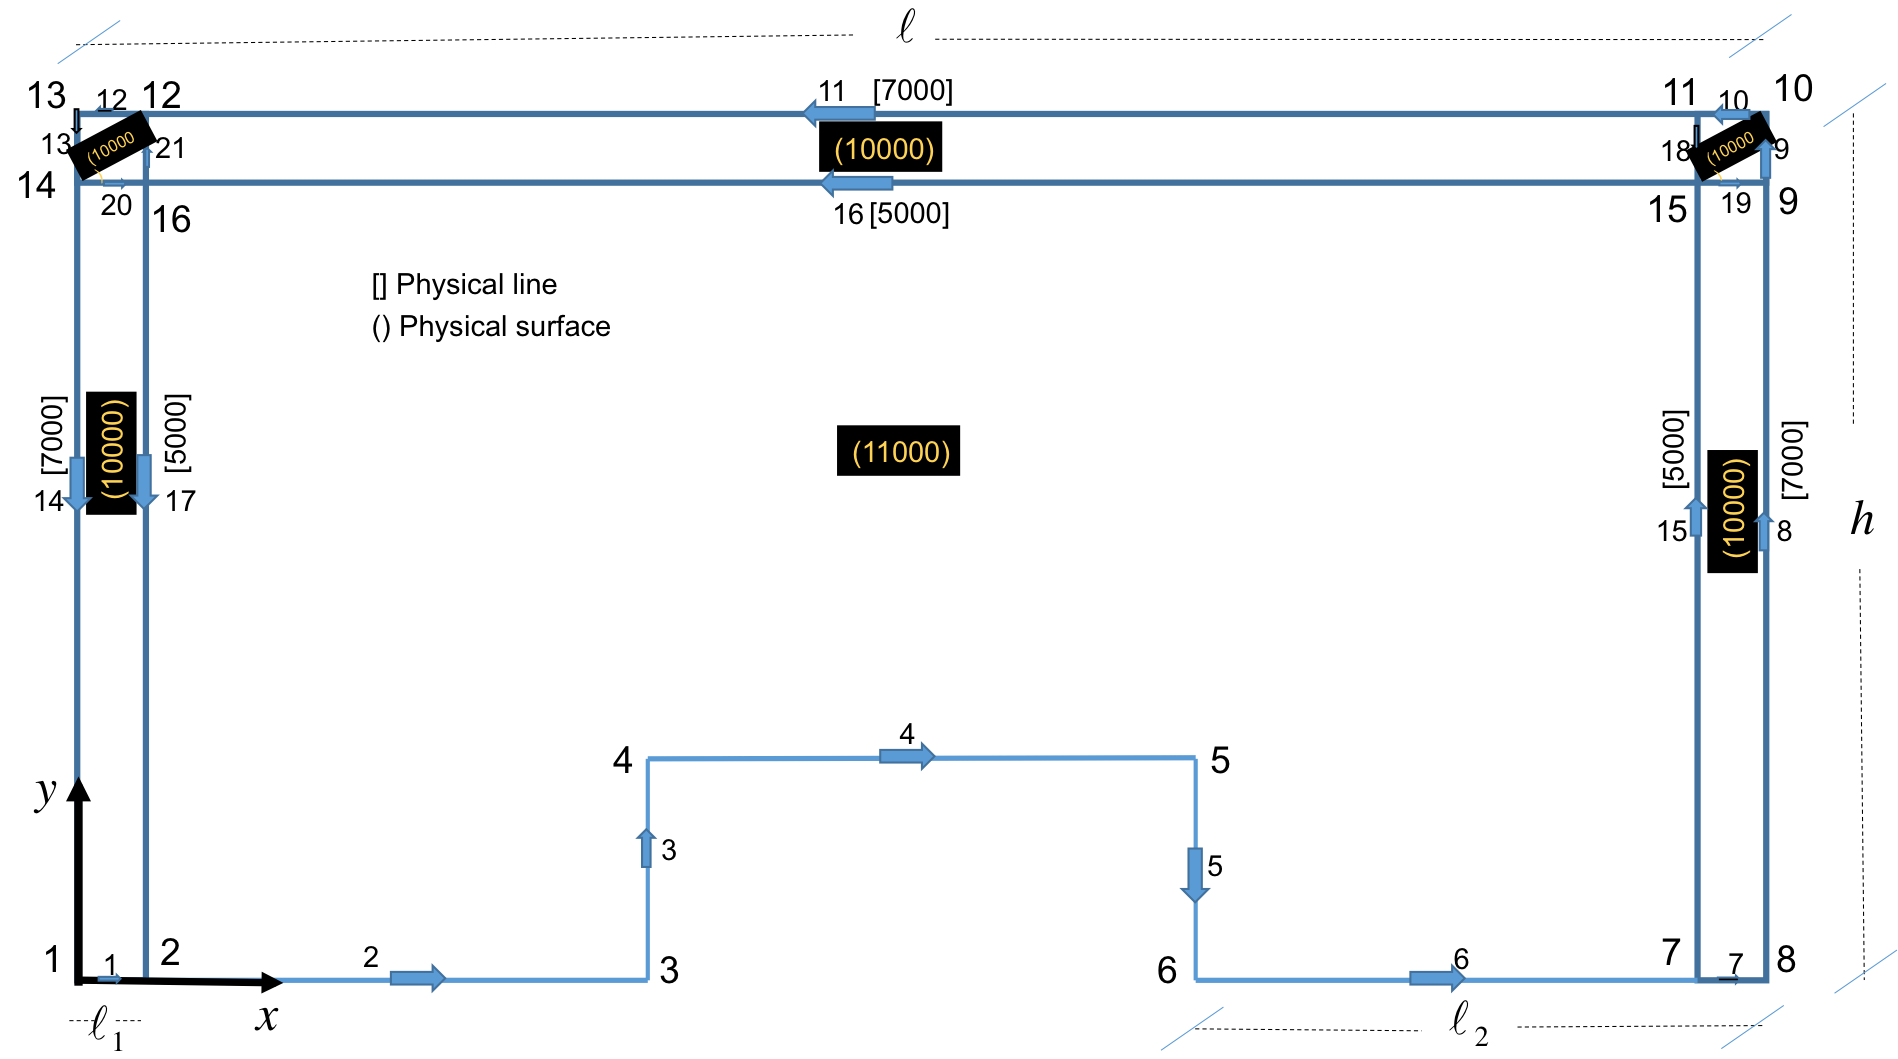
\includegraphics[width=16 cm]{img/plantilla04}}
\caption{Geometry of the general template conformed by a rectangular box used to represent the half-space.}
\label{fig:plantilla2}
\end{figure}


The generalized scatterer is to be subjected to a vertically incident $SV$ plane wave in the form of a Ricker pulse of central frequency $4.0 Hz$, which implies waves of frequencies as large as $16 Hz$ are to be propagated. The half-space has a mass density $\rho = 1.0 Kg-m/m^3$ and a shear wave propagation velocity of $1.0 Km/s$. The characteristic element size is computed as:

\begin{equation}
{h_c} = \frac{{{\beta _{\min }}}}{{12{f_{\max }}}}
\end{equation}

where $\beta_{min}$ is the minimum shear wave propagation velocity in the medium and $f_{max}$ is the largest frequency expected to be propagated. Here we will use characteristic element sizes  of $10$m for the incoming elements and of $25$m for the half-space elements. This is specified in the geometry file {\bf template.geo} by the meshing parameters $cl1 = 0.1$ and $cl2 = 0.25$. Notice that all the dimensions in the .geo file are scaled by a factor of 10 in order to avoid accuracy loss in the resulting mesh. The proper units are recovered in the {\bf node\_write} subroutine of the processing script.

The analysis time step (which is a highly sensitive parameter in the explicit algorithm) is obtained according to:

\begin{equation}
\Delta t = \frac{{{h_c}}}{{10\alpha }}.
\end{equation}

where $\alpha$ is the P-wave propagation velocity. This is specified directly in the header block of the input file by selecting the appropriate time window and number of increments of the analysis. In this case the time span is of $2.0$s divided in $4000$ time steps. In the input file this is specified by the $4001$ value where the extra increment is an algorithmic requirement of the explicit scheme.


\subsubsection*{Th Gmsh .geo file}
The geometry file used to define the model is explained next. In {\bf Gmsh} a model is defined in terms of hierarchical geometric objects like points, lines and plane surfaces. In addition physical objects like physical points, physical lines and physical surfaces can be assigned to the geometric objects in order to facilitate the processing of the {\bf Gmsh} file as required by {\bf WAVES}. The first part of the .geo file describes useful parameters in the model:

\begin{verbatim}
//HEADING BLOCK
//For accuracy all dimensions have been scaled by a factor of 10.0
cl1=0.100;		//Characteristic dimension of the incoming elements. DO NOT MODIFY.
cl2=0.250;		//Characteristic dimension for the elements along other regions
of the domain.
l = 15.0;		//Total domain length.
h =  7.5;		//Total domain height.

l1=0.20;		//Width of the strip. DO NOT MODIFY. THE CODE IS HIGHLY SENSITIVE
 TO THIS PARAMETER
l2=1.00;		//Length of the additional auxiliary line used to decrease the number
of elements.
\end{verbatim}

The next data block defines points required to define the geometry. The fourth parameter in each point definition fixes the target dimension for the elements located in the lines formed by these points.

\begin{verbatim}
//Points
Point(1 ) = {0   , 0   , 0, cl1};
Point(2 ) = {l1  , 0   , 0, cl1};
Point(3 ) = {l2  , 0   , 0, cl2};
Point(4 ) = {l2  , h-l2, 0, cl2};
Point(5 ) = {l-l2, h-l2, 0, cl2};
Point(6 ) = {l-l2, 0   , 0, cl2};
Point(7 ) = {l-l1, 0   , 0, cl1};
Point(8 ) = {l   , 0   , 0, cl1};
Point(9 ) = {l   , h-l1, 0, cl1};
Point(10) = {l   , h   , 0, cl1};
Point(11) = {l-l1, h   , 0, cl1};
Point(12) = {l1  , h   , 0, cl1};
Point(13) = {0   , h   , 0, cl1};
Point(14) = {0   , h-l1, 0, cl1};
Point(15) = {l-l1, h-l1, 0, cl1};
Point(16) = {l1  , h-l1, 0, cl1};
\end{verbatim}

The next hierarchical geometric object correspond to lines which are the union of two or more points. The directional data of each line (see \cref{fig:plantilla2}) must be taken into account in the definition of the plane surfaces, since this data is used to define the element during the meshing process. In {\bf WAVES} the reference system is located along the free surface of the have space with the $y$-axis pointing towards the interior of the half-space. Consequently, the elements are defined in clockwise direction. This convention is usually different from the one implicit in static analysis codes where the elements are defined counterclockwise. In order to keep the same convention the finite element model in {\bf Gmsh} is defined upside-down as shown in \cref{fig:plantilla2} and the plane surfaces must be also defined counterclockwise. This requirement means that a line encountered during the counterclockwise loop is positive if the loop has the same sense as the line and negative otherwise.


\begin{verbatim}
//Lines
Line(1)  = {1 , 2 };
Line(2)  = {2 , 3 };
Line(3)  = {3 , 4 };
Line(4)  = {4 , 5 };
Line(5)  = {5 , 6 };
Line(6)  = {6 , 7 };
Line(7)  = {7 , 8 };
Line(8)  = {8 , 9 };
Line(9)  = {9 , 10};
Line(10) = {10, 11};
Line(11) = {11, 12};
Line(12) = {12, 13};
Line(13) = {13, 14};
Line(14) = {14, 1 };
Line(15) = {7 , 15};
Line(16) = {15, 16};
Line(17) = {16, 2 };
Line(18) = {11, 15};
Line(19) = {15,  9};
Line(20) = {14, 16};
Line(21) = {16, 12};
\end{verbatim}

The next block defines the plane surfaces. A surface is formed by a loop of lines that is traversed in counterclockwise direction. Each surface is identified by an integer number and the Recombine command is issued in order to form quads out of the union of two triangles.



\begin{verbatim}
//Surfaces

//(Right strip)
Line Loop(1) = {7, 8, -19, -15};
Plane Surface(1) = {1};
Transfinite Surface {1} Alternated;
Recombine Surface {1};

// Right strip-lower corner
Line Loop(2) = {9, 10, 18, 19};
Plane Surface(2) = {2};
Transfinite Surface {2} Alternated;
Recombine Surface {2};

//Bottom strip
Line Loop(3) = {-16, -18, 11, -21};
Plane Surface(3) = {3};
Transfinite Surface {3} Alternated;
Recombine Surface {3};


//Left strip-lower corner
Line Loop(4) = {12, 13, 20, 21};
Plane Surface(4) = {4};
Transfinite Surface {4} Alternated;
Recombine Surface {4};

//Left strip
Line Loop(5) = {1, -17, -20, 14};
Plane Surface(5) = {5};
Transfinite Surface {5} Alternated;
Recombine Surface {5};

//Domain enclosed by the strip
Line Loop(6) = {2, 3, 4, 5, 6, 15, 16, 17};
Plane Surface(6) = {6};
//Transfinite Surface {6} Alternated;
Recombine Surface {6};
\end{verbatim}

The final part of the file assigns the physical objects to the different parts of the model. In this case the physical surface $(10000)$ represents the part of the domain where {\bf WAVES} computes only the scattered motion, while in the inside surface identified by the physical surface $(11000)$ {\bf WAVES} computes total motions. The incoming elements will belong to the physical surface $(10000)$  and will have a face in contact with the physical line $[5000]$ representing the scatterer-halfspace interface. The rest of the model is defined by the outer boundary specified by the physical line $[7000]$ where the Lysmer-Khulemeyer absorbing boundaries are to be specified.

\begin{verbatim}
//--------------------
//PHYSICAL SURFACES
//--------------------


// Strip-including its bottom corners
Physical Surface(10000) = {1, 2, 3, 4, 5};

//Domain enclosed by the strip
Physical Surface(11000) = {6};


//--------------------
//PHYSICAL LINES
//--------------------

//Absorbing boundaries
Physical Line(7000) = {8, 9, 10, 11, 12, 13, 14};

//Strip-domain contact surface
Physical Line(5000) = {15 , 16 , 17};
\end{verbatim}

After creating the {\bf .geo} file the next step is meshing the geometry directly from {\bf Gmsh}. The current example uses second order quads.These must be specified in {\bf Gmsh} right after creating the mesh and just before saving the resulting file. All the files for this model are available on the folder {\bf MODELS/[01]TEMPLATE}. However the processing of the {\bf Gmsh} file in order to write the input data file must be conducted in the folder {\bf MODELS/MESHER}. 


\begin{figure}[H]
\centering
\subfloat{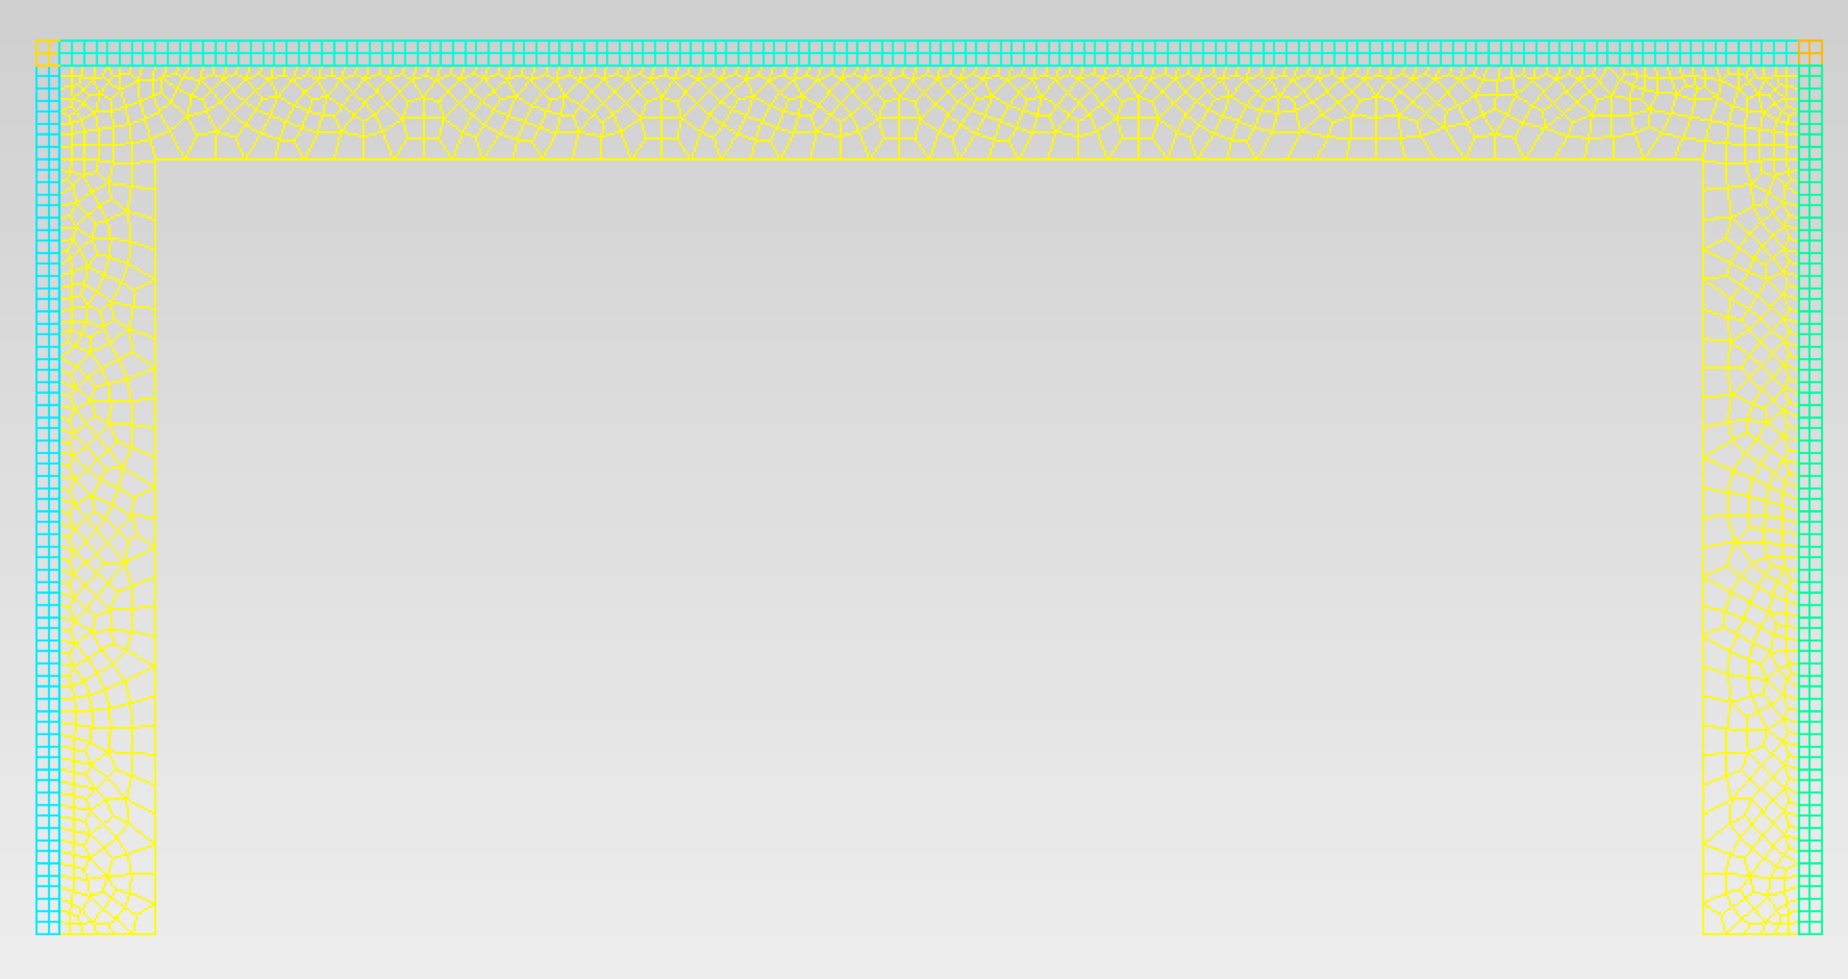
\includegraphics[width=16 cm]{img/malla}}
\caption{Mesh corresponding to the generalized scatterer (template.msh).}
\label{fig:malla}
\end{figure}

\newpage

\subsection*{The mesh processing script}
As pointed out previously the {\bf Gmsh} {\bf template.msh} file must be processed by a python script in order to write the {\bf WAVES} input data file. In this specific example the python script {\bf template\_input.py}, is used to write the {\bf WAVES} data file {\bf template.inp}. The files can be found in the folder {\bf MODELS/[01]TEMPLATE}. 


\subsubsection*{The heading block}
The first part of the script imports the modules {\bf meshio.py} and {\bf mesh\_waves.py} required to read the mesh and the previously described subroutines used to write the data file
\begin{verbatim}
"""
Creates th WAVES.for mesh for a
a generalized scatterer box.
@autor Juan Gomez
"""
from __future__ import division
import meshio
import mesh_waves as msw
import numpy as np
import fileinput
import glob
\end{verbatim}

\subsubsection*{Reading the mesh}
In this part of the script the pyhton-written module meshio reads the {\bf Gmsh} file {\bf template.msh} and stores the model into the dictionaries points, cells, point\_data, cell\_data and field\_data.

\begin{verbatim}
points, cells, point_data, cell_data , field_data = \
    meshio.read("template.msh")
\end{verbatim}
 

\subsubsection*{Processing the nodes}
Now the meshio script creates the array nodes\_array and obtains the total number of nodes in the model. The array is already written in {\bf WAVES} format.
\begin{verbatim}
nodes_array = msw.node_writer(points , point_data)
print len(nodes_array)
\end{verbatim}

\subsubsection*{Processing the elements}
The first surface being processed corresponds to the domain representing the part of the half-space behaving as a scatterer and used mainly to propagate the incident wave from the incoming elements. In the model this corresponds to the physical surface $(11000)$.  The {\bf ele\_writer} subroutine takes as input parameters the python dictionaries storing the mesh, the {\bf Gmsh} element keyword {\bf quad9} identifying the type of elements in the surface, the physical surface tag $(11000)$, the {\bf WAVES} element type code, which in this case corresponds to $9$ for quad9 elements, the material profile tag $5$, the number of nodes and number of degrees of freedom per element and the initial value of the parameter {\bf nini=0}. After processing the first physical surface the subroutine returns the total number of elements in the set with the parameter {\bf nfin} and the first array of elements array {\bf els1\_array}.

The next part of the script takes care of the surface containing the incoming elements. The subroutine is initialized with the final value of the element counter resulting from the previous surface {\bf nini = nfin}. The remaining two parameters correspond to the physical surface $(10000)$ and to the physical line $[5000]$ identifying the interface between the half-space and the strip of incoming elements. By default incoming elements are quad9 and this is already considered in the subroutine. In this case the information corresponding to the physical surface $(10000)$ is stored in the elements array  {\bf els2\_array}.

In the final part of the elements block the script process the absorbing boundary. In this case the routine {\bf boundary\_writer} requires as input parameter the initial value of the elements counter {\bf nini = nfin}, the physical line identifying the absorbing boundary $[7000]$ and the {\bf WAVES} code $6$ identifying the element type. The resulting elements array in {\bf WAVES} format  is now stored in {\bf els3\_array}. 

\begin{verbatim}
nfin , els1_array  = msw.ele_writer(cells , cell_data , 'quad9' , 11000 , 3 , 5 ,
                                                        18 , 9 , 0 )
nini = nfin
nfin , els2_array  = msw.face_recognition(cells , cell_data , 10000 , 5000 , nini)
nini = nfin
nfin , els3_array  = msw.boundary_writer(cells , cell_data , 7000 , 6 , nini)
\end{verbatim}

\subsubsection*{Writing the template.inp file}
In the final part of the script the code writes the nodes and elements arrays into text files and then links all the files into a single .inp file with the name {\bf template.inp}. The numbers 2 trhough 7 in the text files are used to ensure that the final .inp file is assembled in that order. In this case it has been assumed that the user has independently created a file starting by 1, which in this case corresponds to the file {\bf 1header.txt} and a file number 3 corresponding to the material block given by the file {\bf 3mater.txt}.

\begin{verbatim}
np.savetxt("2nodes.txt", nodes_array,
           fmt=("%d", "%d", "%d" , "%d" , "%.4f", "%.4f"))
np.savetxt("5eles.txt", els1_array   , fmt="%d")
np.savetxt("6eles.txt", els2_array   , fmt="%d")
np.savetxt("7eles.txt", els3_array   , fmt="%d")


file_list = glob.glob("*.txt")

with open('template.inp', 'w') as file:
    input_lines = fileinput.input(file_list)
    file.writelines(input_lines)
\end{verbatim}

Before executing the script the user must create the header and the material files {\bf 1header.txt} and {\bf mater.txt}. Th first file contains the general model data while the second file contains the different material profiles for the specific model. The construction of both data blocks is explained in the next section.

After the solution is complete the following solution can be visualized using {\bf Paraview}:


\begin{figure}[H]
\centering
\subfloat{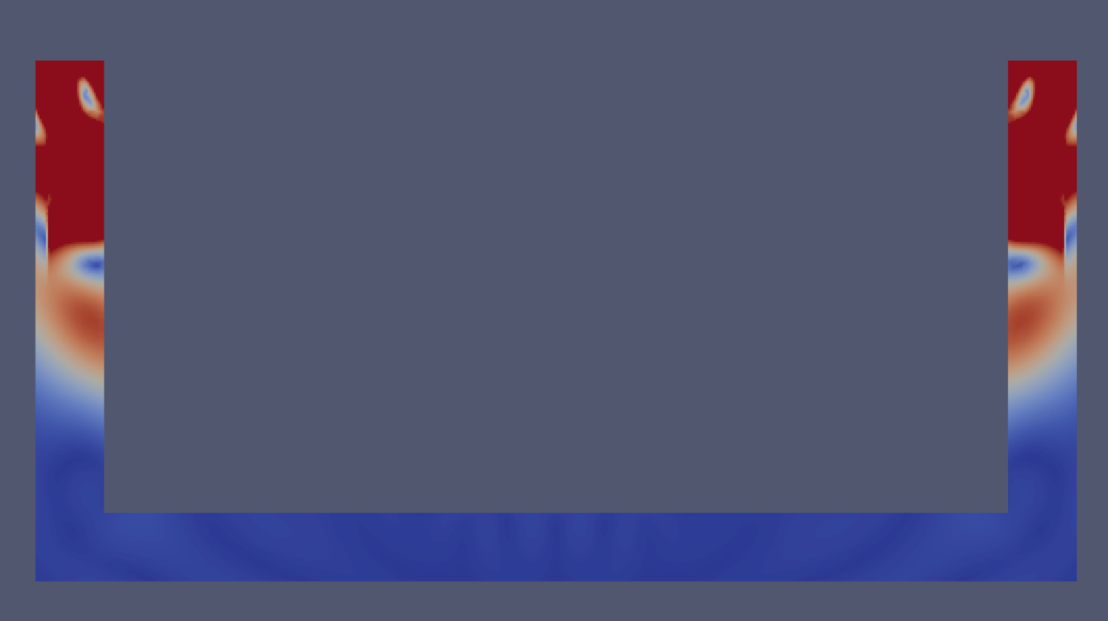
\includegraphics[width=16 cm]{img/video}}
\caption{Snapshot of the solution at a particular time instant. The full video is available in the folder {\bf MODELS/[01]TEMPLATE }.} 
\label{fig:malla}
\end{figure}
 
\subsubsection*{Structure of the {\bf *.inp} file}
This data file is defined as follows:

\begin{verbatim}
--------------------------------------
------------HEADING BLOCK-------------
--------------------------------------
Title
NNODES     NUMEL   NMAT   Tm  NINCS    NDIM    NMNE    NMDOFE     NMRMAT
NMIMAT     NPLOADS     IMODE    NOUTPU
NSNAP  NPROCESS

NNODES  : Total number of nodes.
NUMEL   : Total number of elements.
NMAT    : Total number of material profiles.
Tm      : Duration of the analysis.
NINCS   : Total number of increments.
NDIM    : Problem dimensionality.
NMNE    : Maximum number of nodes per element.
NMDOFE  : Maximum number of degrees of freedom per element.
NMRMAT  : Maximum number of real material properties in a given profile.
NMRMAT  : Maximum number of integer material properties in a given profile.
NPLOADS : Number of point loads.     
IMODE   : Point load application mode (0 for Ricker pulse; 1 for an input file)    
NOUTPU  : Number of points where output is required.
NSNAP   : Snapshot increment for the creation of VTK fils.
NPROCESS: Number of processors.
--------------------------------------
------------NODAL BLOCK---------------
--------------------------------------
As many data lines as specified by NNODES with the following data:
ID_NODE NDOF  BC-1   BC-2....BC-NDOF   X-coord    Y-coord
ID_NODE  :Nodal identifier. 
NDOF     :Number of degrees of freedom at the current node.  
BC-1   BC-2....BC-NDOF:Boundary condition flag for each one of the NDOF degrees
of freedom (0 free; 1 restrained)   
X-coord  :X-coordinate of the current node.    
Y-coord  :Y-coordinate of the current node.
----------------------------------------
------------MATERIAK BLOCK--------------
----------------------------------------
As many data lines as specified by NMAT with the following data:
MAT_ID     NMRMAT   NMIMAT    Par-1   Par-2...Par-NRMAT    IPAR-1
IPAR-2...IPAR-NMIMAT
MAT_ID   :Material profile identifier.
NMRMAT   :Number of real material properties for this profile.   
NMIMAT   :Number of integer material properties for this profile.    
Par-1   Par-2...Par-NRMAT    :Real material properties. (In a classic 2D wave
propagation analysis the parameters are P-wave velocity; SV wave velocity;
mass density; alpha Rayleigh damping parameter; Beta Rayleigh damping
parameter)
IPAR-1   IPAR-2...IPAR-NMIMAT:Integer material properties.
(This is used in the definition of incoming elements
in order to specify the face in contact with the scatterer).
Profiles 1 through 4 are reserved for incoming elements.      
----------------------------------------
------------WAVE BLOCK------------------
----------------------------------------
1 data line with the following wave information:
IWAVE     Tm     Tini     fc     Amp    Phi
IWAVE    :Wave type index (1 for SV;2 for P wave).    
Tm       :Time span of the analysis in the case of a Ricker pulse.     
Tini     :Initial time of the Ricker pulse.     
fc       :Central frequency of the Ricker pulse.     
Amp      :Amplitude of the incident wave.    
Phi      :Incidence angle of the plane wave.
----------------------------------------
------------ELEMENTS BLOCK--------------
----------------------------------------
As many data lines as specified by NUMEL each one with the following data:
ID_ELE  ELETYPE  NDOFE     MAT_TAG   NNODES   N1   N2   N3....N-NNODES
ID_ELE  :Element id.
ELETYPE :Element type.
NDOFE   :Number of degrees of freedom at the element.
MAT_TAG :Material profile assigned to the element.
NNODES  :Number of nodal points for the element.
N1   N2   N3....N-NNODES: NNODES-nodal points for the element.
----------------------------------------
------------LOADS BLOCK-----------------
----------------------------------------
As many data lines as loaded nodal points.
ID_NODE   ID_DOF
ID_NODE   :Id of the loaded node.
ID_DOF    :Degree of freedom of the point load.
----------------------------------------
------------OUTPUT BLOCK----------------
----------------------------------------
As many data lines as defined by NOUTPU each one indicating
a nodal identifier at which the output history is required.
\end{verbatim}


\section{Running the program}
To execute {\bf WAVES} use the following command at the terminal window:

\begin{verbatim}
./waves.out
\end{verbatim}
 
 
\begin{figure}[H]
\centering
\subfloat{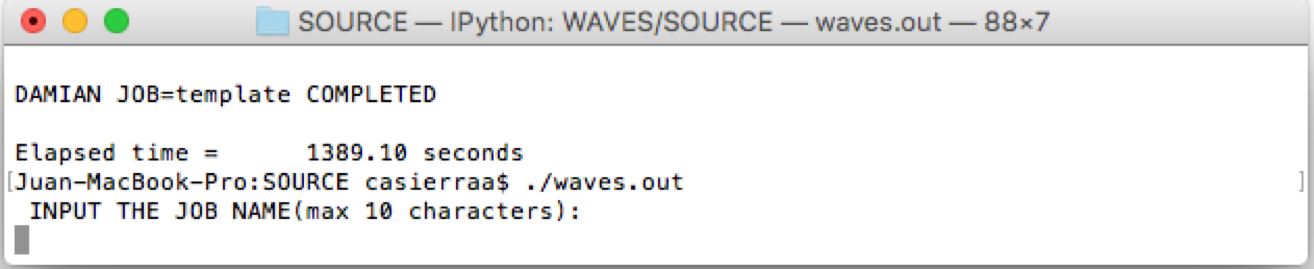
\includegraphics[width=16 cm]{img/terminal}}
\caption{Running WAVES from the terminal window.}
\label{fig: terminal}
\end{figure} 
 
and input the name of the data file (without extension). If the analysis is finished successfully you will get the following output:

\begin{figure}[H]
\centering
\subfloat{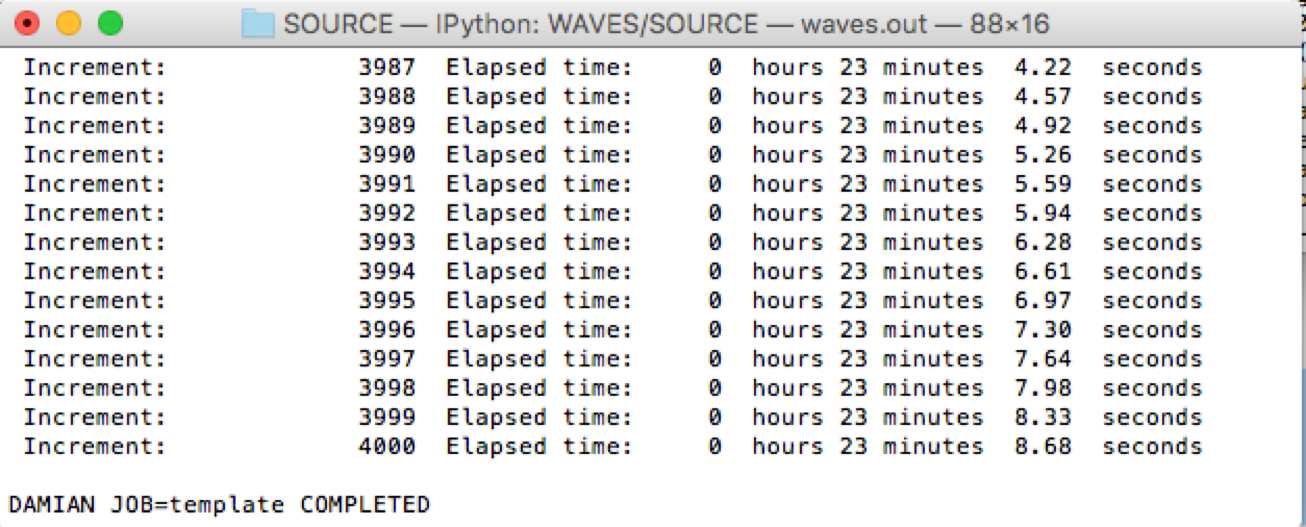
\includegraphics[width=16 cm]{img/complete}}
\caption{Running WAVES from the terminal window.}
\label{fig: terminal}
\end{figure} 
 
The displacement solution can be visualized with {\bf PARAVIEW} by opening the response files {\bf Body\_Txx.vtk} which are written into the folder {\bf SOURCE/vtk}


\bibliographystyle{gji}
\bibliography{references}
\phantomsection
\addcontentsline{toc}{section}{REFERENCES}


 
\end{document}